% !TEX encoding = UTF-8
% !TEX TS-program = pdflatex
% !TEX root = ../nt.tex
% !TEX spellcheck = it-IT

%************************************************
\chapter{TEORIA DELLE CODE}
\label{cap:qtheory}
%************************************************\\

\section{PROCESSI STOCASTICI}

Modello matematico di tipo probabilistico utilizzato per andare a descrivere dei fenomeni casuali che possono essere rappresentati come funzioni di un parametro che solitamente è il tempo. $\{X(t),\ t \in T\}$. Famiglia di variabili casuali $X(t)$, indicizzate dal parametro temporale $t \in T$. Potrebbe anche essere qualche altra grandezza. Le v.a. sono definite su un unico spazio campione e che assumono valori in un certo insieme $S$. I valori assunti sono detti stati. $S$ = spazio degli stati del processo. Un processo stocastico è un insieme di funzioni del tempo. $X(t)$ generica variabile casuale. $X(t)\ \in S$. Insieme di funzioni del tempo che vengono chiamate \textbf{Realizzazioni}. Spazio campione: possibili risultati.

$X(t): T \mapsto S$ SAMPLE PATHS: realizzazioni. La cosa importante è che $X(t)$ è completamente specificato in termini probabilistici se posso scrivere la CDF congiunta (e la PDF). $X(t)$ famiglia di variabili casuali. Differenti realizzazioni. Un processo stocastico è completamente specificato con la CDF congiunta per un qualsiasi insieme (sottoinsieme) di v.a. estratte dal processo. Immaginiamo di estrarre $n$ variabili casuali:

$X(t_i),\ i=1,2,\dots,n$: estrazione di $n$ variabili casuali. Per queste devo essere in grado di scrivere la CDF congiunta:

\[
	F_{\mathbf{\underline{X}}}(\underline{x}; t) := \Pr\{X(t_1) \leq x_1,\ X(t_2) \leq x_2,\ \dots,\ X(t_n) \leq x_n\}
\]

Tale è la CDF CONGIUNTA. Ricordiamo che data una variabile casuale $\xi$, abbiamo che: $F_{\xi}(t) := \Pr\{\xi\leq t\}$. 
Qui bisogna riuscire la scrivere la CDF congiunta per queste $n$ variabili casuali estratte dal processo. In alternativa, potrei considerare la PDF congiunta, la quale è la derivata della CDF. Scriviamo la \textit{ROW VECTOR NOTATION}, generalizzando le casistiche dimensionali:

\[
	\left\{
	\begin{aligned}
	&\mathbf{\underline{X}} = (X(t_1),\ X(t_2),\ \dots,\ X(t_n)) \in\R^{n\times 1}  \\
	&\underline{x} = (x_1,\ x_2,\ \dots,\ x_n) \in\R^{n\times 1}\\
	&\underline{t} = (t_1,\ t_2,\ \dots,\ t_n) \in\R^{n\times 1}
	\end{aligned}
	\right.
\]

Ricordiamo, ancora: $[f_{\mathbf{\underline{X}}}(\underline{x}; t) = \frac{\partial{F_{\mathbf{\underline{X}}}(\underline{x}; t)}}{\partial{\underline{x}}}]$.

\subsection{CATENE DI MARKOV}

Pensiamo allo spazio degli stati $S$. Questo spazio può essere continuo o discreto. Una CATENA è un processo stocastico a stato discreto. Noi tratteremo le \textit{\textbf{CATENE DI MARKOV}}. $t$ può essere continuo o discreto. Tempo continuo o tempo discreto, rispettivamente. Quando il tempo è discreto, si parla di \textit{SEQUENZA STOCASTICA}. Eventualmente potremmo avere: $X_n,\ n=0,1,2,\dots$ ovvero diverse componenti del sistema.

Noi studieremo le CATENE DI MARKOV a tempo continuo, dette \underline{CMTC}. Categoria di processi stocastici. Per questi processi di MARKOV la relazione che intercorre tra le v.a. è molto semplice. Caratterizzazione molto semplice. Questi processi soddisfano la cosiddetta:

\begin{defn}{\textbf{PROPRIET\`A DI MARKOV}}

\[
	\Pr\{X(t) \leq x\ |\ X(t_n) = x_n,\ X(t_{n-1}) = x_{n-1},\ \dots,\ X(t_0) = x_0\} = \Pr\{X(t) \leq x\ |\ X(t_n) = x_n\}
\]

con $t > t_n > t_{n-1} >\ \dots\ > t_0$. 
\end{defn}

Questo è un processo stocastico $\{X(t),\ t\in T\}$ che soddisfa alla proprietà di MARKOV. Si tratta di una CDF condizionata. Cosa mi dice? L'evoluzione futura del processo a partire dall'istante $t_n$ non dipende dalla storia passata ma solo dallo stato finale del processo! L'evoluzione del processo da $t_n$ in poi dipende soltanto da $t_n$. Lo stato in $t_n$ riassume tutta la storia passata del processo. $\{X(t),\ t\in T\}$. Noi studieremo le catene di Markov a tempo continuo (stato discreto, tempo continuo). 

\begin{defn}{\textbf{CM omogenea}}

Invariante rispetto a traslazioni temporali degli assi:

\[
	\Pr\{X(t) \leq x\ |\ x(t_n) = x_n\} = \Pr\{X(t-t_n) \leq x\ |\ X(0) = x_n\}
\]

con $t > t_n$.
\end{defn}

Sono sostanzialmente delle catene per modellare sistemi il quale comportamento NON dipende dal tempo di osservazione. Scelta possibile dell'arco temporale. \underline{OMOGENEIT\`A}.

\begin{defn}{\textbf{COIMPLICAZIONE DELLA PROPRIET\`A DI MARKOV (\textit{tempo di soggiorno})}}

$W_i,\ i\in S$. Uno stato i qualsiasi della mia catena dev'essere una v.a. priva di memoria. Quando una v.a. casuale soddisfa alla proprietà di assenza di memoria, vale il seguente:

\[
	[\Pr\{W_i > t+\tau\ |\ W_i > t\} = \Pr\{W_i > \tau\}]
\]

Tale è la \textit{MEMORYLESS PROPERTY}.
\end{defn}

Se l'evoluzione futura del processo a partire da $t_n$ non dipende dallo stato passato del processo, non dipenderà neanche dal tempo in cui ci è stato. L'unica distribuzione di v.a. continua che soddisfa alla proprietà di assenza di memoria è la

\begin{defn}{\textbf{ESPONENZIALE NEGATIVA UNILATERA}}

\[
	\left\{
	\begin{aligned}
	&[\underline{f_{W_i}(\tau) = a\e^{-a\tau},\ \tau \geq 0}]\\
	&\left\{
	\begin{aligned}
	&F_{W_i}(\tau) = \Pr\{W_i\leq\tau\} = 1-\e^{-a\tau},\ \tau\geq 0\\
	&F_{W_i}^c(\tau) = \Pr\{W_i\geq\tau\} = \e^{-a\tau},\ \tau\geq 0
	\end{aligned}
	\right.
	\end{aligned}
	\right.
\]

\end{defn}

Unica distribuzione di probabilità che soddisfa l'assenza di memoria. Vedremo in seguito come $a := -q_{ii}$ (velocità totale di uscita dallo stato i). Velocità o equivalentemente tasso di transizione.

Proprietà di assenza di memoria per una v.a. casuale (in particolare comporta conseguenze sul tempo di soggiorno in uno stato $i$ di una CMTC):

\[
	\Pr\{W_i > t+\tau\ |\ W_i > t\} = \Pr\{W_i > \tau\}
\]	
	
Parliamone in generale.

\begin{thrm}
L'unica PDF di una v.a. continua che soddisfa alla proprietà di ASSENZA di MEMORIA è l'ESPONENZIALE NEGATIVA UNILATERA (UEN). 
\end{thrm}

\begin{proof}{\textbf{UEN MEMORYLESS PROPERTY}}
\[
	\Pr\{W_i > t+\tau\ |\ W_i > t\} = \frac{\Pr\{W_i > t+\tau,\ W_i > t\}}{\Pr\{W_i > t\}} =(\dots)
\]

Dobbiamo dimostrare questa proprietà per la UEN: $W_i>t+\tau\supseteq W_i>t \implies$

\[ 	
	(\dots) = \frac{\Pr\{W_i > t+\tau\}}{\Pr\{W_i > t\}} = \frac{\e^{-a(t+\tau)}}{\e^{-at}} = \frac{\e^{-at}\e^{-a\tau}}{\e^{-at}} = \e^{-a\tau} = \underline{\Pr\{W_i > \tau\}}
\]

La parte sottolineata sarebbe quindi la CDF complementare $F_{W_i}^c(\tau)$ della UEN.
\end{proof}

A cosa è uguale il parametro $a$? \`E uguale ad $a = -q_{ii}$, che sarebbe la velocità (totale) di uscita dallo stato $i$, ovvero la velocità totale alla quale il processo cerca di uscire dallo stato $i$. Si scrive, posto $a := -q_{ii}$:

\[
	W_i \sim EXP(-q_{ii}),\ \forall i\in S
\]

Quindi il sistema precedente diventa:

\[
	\left\{
	\begin{aligned}
	&[f_{W_i}(\tau) = -q_{ii}\e^{q_{ii}\tau},\ \tau \geq 0]\\
	&\left\{
	\begin{aligned}
	&F_{W_i}(\tau) = \Pr\{W_i\leq\tau\} = 1-\e^{q_{ii}\tau},\ \tau\geq 0\\
	&F_{W_i}^c(\tau) = \Pr\{W_I\geq\tau\} = \e^{q_{ii}\tau},\ \tau\geq 0
	\end{aligned}
	\right.
	\end{aligned}
	\right.
\]

La proprietà di assenza di memoria per $W_i$ dice che, supponendo che il processo stia soggiornando sullo stato i da $t$ unità di tempo, la probabilità che il processo mi soggiorni ancora per altre $\tau$ unità di tempo è pari alla probabilità che il processo soggiorni per $\tau$ unità di tempo. Posto $\tau$ = RESIDUO, definiamo $\Phi_{i,t}$ come tempo di soggiorno residuo nello stato i da $t$ unità di tempo, ovvero il processo si trova già da $t$ unità di tempo nello stato i! Quindi riscriviamo la MLP.

\begin{corl}

\[
	\Pr\{\Phi_{i,t} > \tau\} = \Pr\{W_i > \tau\}
\]

La distribuzione del tempo di soggiorno residuo in un tempo $t$ (LHS) è pari alla distribuzione del tempo di soggiorno (RHS). 

\[
	\left\{
	\begin{aligned}
	&[(W_i \sim \Phi_{i,t}) \sim EXP(-q_{ii})]\\
	&f_{\Phi_{i,t}}(\tau) = -q_{ii}\e^{q_{ii}\tau},\ \tau\geq 0
	\end{aligned}
	\right.
\]

\end{corl}

Nel tempo discreto la distribuzione che soddisfa la MLP è solo quella geometrica. Noi invece lavoriamo a tempo continuo. MARKOVIANIT\`A: assenza di memoria nel processo markoviano. Tempo di soggiorno residuo e tempo di soggiorno non solo hanno la stessa medesima distribuzione esponenziale (UEN), ma sono distribuite anche con lo stesso parametro $-q_{ii} = a$!

Riscriviamo la proprietà di Markov a tempo continuo! (specializzazione): Stiamo lavorando con \underline{CMTC} o CTMC (Continuos Time Markov Chain):

\[
	\Pr\{X(t_{n+1}) = x_{t_{n+1}}\ |\ X(t_n) = x_n,\ X(t_{n-1}) = x_{n-1},\ X(t_0) = x_0\} =
\]
\[
	= \Pr\{X(t_{n+1}) = x_{t_{n+1}}\ |\ X(t_n) = x_n\}
\]

$\forall x_k \in S,\ t_{n+1} > t_n > t_{n-1} >\ \dots\ > t_0$.

Chiamiamo il secondo membro \underline{probabilità di transizione}: $[\Pr\{X(t_{n+1}) = x_{n+1}\ |\ X(t_n) = x_n\}]$. Supponendo che nel tempo $t_n$ il processo si trovi in $x_n$, essa è la probabilità che al tempo $t_{n+1}$ si trovi allo stato $x_{n+1}$. Ma essa non fornisce informazioni circa quello che potrebbe accadere nel frattempo tra $t_n$ e $t_{n+1}$!

\begin{defn}{\textbf{Probabilità di Transizione da i a j}}
\[
	[\underline{p_{ij}(t,\theta) := \Pr\{X(\theta) = j\ |\ X(t) = i\}}]
\]
\end{defn}

$\forall i,j\in S$, e supponendo naturalmente che $\theta > t$.

Se la CMTC è OMOGENEA, queste probabilità di transizione non dipendono dagli istanti di tempo, ma dalla differenza dei due istanti di tempo $[\tau := \theta-t]$.

\[
	[p_{ij}(t,\theta) := \underline{P_{ij}(\tau)} = \Pr\{X(t+\tau) = j\ |\ \underline{\underline{X(t) = i}}\}]
\]

Supponendo che all'istante di tempo $t$ lo stato sia i, quella è la probabilità che dopo $\tau$ istanti di tempo lo stato sia j. Non ci riferiamo più necessariamente ai singoli istanti di tempo. Vale: $[\sum_{j\in S}{p_{ij}(\tau)} = 1]$. Distribuzione al tempo $t$: intendiamo l'insieme di queste probabilità:

\begin{defn}{\textbf{Distribuzione al tempo t}}

\[
	\pi_i(t) := \Pr\{X(t) = i\}\ \forall i\in S
\]
\end{defn}

Andiamo a considerare tutti gli stati del mio processo. Per il teorema delle probabilità totali questa probabilità la posso scrivere in tal modo:

\[
	\pi_i(t) := \Pr\{X(t) = i\} = \sum_{j\in S}{\Pr\{X(t) = i\ |\ X(0) = j\}\Pr\{X(0) = j\}} = \sum_{j\in S}{\underline{p_{ji}(t)}\underline{\pi_j(0)}}
\]

Quindi questa distribuzione al tempo $t$ la possiamo ottenere come somma di prodotti tra la distribuzione iniziale e la probabilità di transizione da j ad i. Possiamo inoltre, dato $\pi_j(0)$, conoscere qualsiasi CDF congiunta. Per ogni processo particolare posso scriverle facilmente... A tempo continuo le probabilità di transizione dipendono però dal tempo! $(\dots) = \mathord{\cdot}(t)$! Per semplificare la vita, sono state introdotte delle quantità legate a $\underline{p_{ji}(t)}$, generalmente anch'esse dipendenti dal tempo, ma che, nel caso in cui la CMTC sia OMOGENEA, sono invece costanti. Queste quantità sono quindi costanti e sono chiamate TASSI o \textit{VELOCIT\`A DI TRANSIZIONE}. Ciò che NON è costante è invece la probabilità di transizione.

\subsubsection{Tassi di Transizione}

\begin{defn}{\textbf{TASSI (o VELOCIT\`A) di transizione}}

Relazione che lega i tassi di transizione alle probabilità di transizione.
Se la catena è regolare:

\[
	\left\{
	\begin{aligned}
	&\exists q_{ij} := \lim_{\Delta t\to 0}{\frac{p_{ij}(\Delta t)}{\Delta t}},	\forall (i\neq j)\in S\\
	&\exists q_{ii} := \lim_{\Delta t\to 0}{\frac{p_{ii}(\Delta t)-1}{\Delta t}} \leq 0
	\end{aligned}
	\right.
\]

$\forall i,j\ \in S$.
\end{defn}

Si può dimostrare che questi limiti, queste quantità, esistono se la CMTC è REGOLARE, ovvero se:

\begin{defn}{\textbf{CMTC REGOLARE}}

\[
	\forall X(0),\ [\underline{\cardinality{transizioni(\Delta t < +\infty)} < +\infty}]
\]
\end{defn}

Questo deve valere per qualunque stato iniziale. $-q_{ii} \geq 0$. Supponiamo che lo stato del processo in $t$ sia $i$ $\iff X(t) = i$. La probabilità che in un intervallo $\Delta t$ tendente a 0 ($\iff \Delta t \to 0$) vi sia una transizione al di fuori di i è: $[-q_{ii}\Delta  t + o(\Delta t)]$.
Ragioniamo invece su $p_{ii}(\Delta t)$: essa rappresenta la probabilità che lo stato presente sia $i$ e tra $\Delta t$ unità di tempo lo stato sia di nuovo $i$. Tale probabilità non mi dice nulla su tutte le possibili transizioni che ci possono essere tra $t$ e $t+\Delta t$.

$1-p_{ii}(\Delta t),\ \Delta t \to 0$ è la probabilità che dopo $\Delta t$ unità di tempo lo stato NON sia più $i$, partendo da $i$ (prob. che vi sia una transizione). Quando $\Delta t \to 0$, questa probabilità tende alla probabilità di leaving dallo stato $i$. Quindi invertendo la seconda equazione del precedente sistema troviamo che al limite essa è uguale a: $[-q_{ii}\Delta t + o(\Delta t)]$. La probabilità è tanto più grande quando $q_{ii}$ è alto in modulo! Più velocemente esce, più è probabile che esca! Più grande è il valore $\abs{q_{ii}}$, più il processo cerca di uscire velocemente, e quindi con maggior probabilità vi riuscirà $\implies \abs{q_{ii}} \uparrow \implies$ processo più velocemente tende ad uscire.

$-q_{ii}$ è quindi la velocità alla quale un processo lascia lo stato $i$. In sostanza, $-q_{ii}$ rappresenta il numero medio di transizioni al di fuori di $i$ $\forall$ unità di tempo \newline
\underline{in cui il processo si trova nello stato $i$}.

Prendiamo per esempio due diverse realizzazioni dello stesso processo: $\{X^{(1)}(t),\ X^{(2)}(t)\}$. Per $X^{(1)}(t)$ abbiamo diversi soggiorni nello stato i. Supponiamo che la somma delle durate di soggiorno in $i$ facciano $1s$. Durante questa unità di tempo in cui il processo si trova in $i$, si trovano 7 transizioni al di fuori di $i$. Per $X^{(2)}(t)$, supponiamo lo stesso caso ma con 5 transizioni. Abbiamo detto che: $-q_{ii}$ è il numero medio di transizioni al di fuori dello stato $i$. Una transizione uscente segue un \underline{tempo di soggiorno}. $-q_{ii}$ rappresenta quindi anche il tempo medio di soggiorno. Ricordando che $f_{W_i}(\tau) = -q_{ii}\e^{q_{ii}\tau}$, abbiamo che:

\[
	\E[W_i] = \frac{1}{-q_{ii}}
\]

Se calcoliamo il valor medio (la media) di $f_{W_i}(\tau)$, esce proprio $(\frac{1}{-q_{ii}})$; tanto più grande è $q_{ii}$, tanto basso sarà il tempo di soggiorno in media.

Significato di $q_{ij}$. Supponiamo che attualmente il processo si trovi in $i$. La probabilità che in un intervallo di tempo infinitesimo ($\Delta t \to 0$) vi sia una transizione $ij$, ($i \rightarrow j$), è uguale alla probabilità $q_{ij}\Delta t + o(\Delta t)$. Consideriamo $p_{ij}(t)$. Non mi dice nulla, essendo una probabilità di transizione, su cosa sia eventualmente accaduto nel rispettivo intervallo di tempo tra la transizione.

Accade quindi che:

\[
	[\lim_{\Delta t \to 0}{\frac{p_{ij}(t)}{\Delta t}} = q_{ij}]
\]

(probabilità tanto più grande quanto più grande è $q_{ij}$).
La velocità è $q_{ij}$. Rappresenta una velocità alla quale si verifica la transizione $i \rightarrow j$. Ecco perché viene detto TASSO (o VELOCIT\`A) di TRANSIZIONE da $i$ a $j$. Ma è anche in sostanza il numero medio di transizioni da $i$ a $j$ $(i \rightarrow j) \ \forall$ unità di tempo in cui il processo si trova nello stato i$i$ Ragioniamo di nuovo sulle due funzioni rappresentanti due diverse realizzazioni dello stesso processo. Supponiamo sempre che la durata complessiva di un soggiorno in $i$ sommi temporalmente ad 1. $q_{ij}$ si differenzia da $-q_{ii}$ in quanto rappresenta il numero medio di transizioni ($i \rightarrow j$).

\[
	\sum_{(j\neq i)\in S}{q_{ij}} = \sum_{(j\neq i)\in S}{(\lim_{\Delta t \to 0}{\frac{p_{ij}(\Delta t)}{\Delta t}})} = \lim_{\Delta t \to 0}{\sum_{(j\neq i)\in S}{(\frac{p_{ij}(\Delta t)}{\Delta t})}} = (\dots)
\]

Considerando uno stato $i$ qualsiasi, questa sommatoria fa 1: $\iff \sum_{j\in S}{p_{ij}(\Delta t)} = 1$. Quindi:

\[
	(\dots) = \lim_{\Delta t \to 0}{\frac{1-p_{ii}(\Delta t)}{\Delta t}} = \underline{\underline{-q_{ii}}}
\]

La quale è la velocità \underline{totale} di uscita dallo stato $i$. Introduciamo ora una seconda quantità: $[\tau_{i,j} = \frac{q_{ij}}{-q_{ii}}]$, ovvero la probabilità che il processo, lasciando lo stato i, faccia una transizione verso lo stato $j$. 

Supponiamo che $q_{ij}=10,\ q_{ik}=30,\ q_{ih}=60$... mediamente vi siano quindi 100 transizioni uscenti. $-q_{ii} = \sum_{(j\neq i)\in S}{q_{ij}} = 100$. Abbiamo che:

\[
	\left\{
	\begin{aligned}
	&\tau_{i,j} = \frac{10}{100} = 0.1\\
	&\tau_{i,h} = \frac{60}{100} = 0.6\\
	&\tau_{i,k} = \frac{30}{100} = 0.3
	\end{aligned}
	\right.
\] 

$\tau_{i,j}$ è quindi alla fine la probabilità che, supponendo di lasciare $i$, la transizione sia verso $j$. LASCIANDO LO STATO $i$, $\exists$ UNA TRANSIZIONE VERSO LO STATO $j$.

Distribuzione al tempo $t$. Ci sono dei sistemi di equazioni differenziali che legano la distribuzione al tempo $t$ ai tassi di transizione:

\[	
	\left\{
	\begin{aligned}
	&\underline{\pi_i}(t) := \Pr\{X(t) = i\},\ \forall i\in S\\
	&\frac{d \pi_i(t)}{dt} = \sum_{j\in S}{q_{ji}\pi_j(t)},\ \forall i\in S
	\end{aligned}
	\right.
\]

Di queste equazioni differenziali ve n'è una $\forall s\in S$ della nostra catena. Nella maggior parte dei casi, non ci serve $\pi_i(t)$, ma una distribuzione a regime (costante). A regime serve la rispettiva distribuzione a regime (dopo un tempo molto grande). Ci sono delle condizioni in base alla quale $\pi_i(t) \to K \neq \mathord{\cdot}(t)$ (distribuzione di equilibrio, a regime). Ma quali sono queste condizioni?

\subsection{Probabilità a regime}

Quali sono le condizioni di esistenza delle probabilità di stato a regime? Introduciamo alcune definizioni. Consideriamo uno stato $i \in S$ della mia \underline{CMTC}. Diciamo che lo stato $(i\in S)$ è \textit{TRANSITORIO} se c'è una probabilità non nulla che il processo non torni più in quello stato dopo che esso viene lasciato. Si dirà \textit{RICORRENTE} in caso contrario (se con probabilità 1 torni nello stato $i$ dopo averlo lasciato). Ai fini della distribuzione di regime, a noi interessano i RICORRENTI (gli stati ricorrenti). Sia $M_i$ il tempo medio di ritorno (o \underline{di ricorrenza} nello stato $i$). Per tempo di ritorno si intende il tempo che passa da \underline{due ingressi consecutivi} nello stato $i$. $M_i$ dice quanto dura in media questo tempo (ovviamente guardando tutte le possibili realizzazioni, altrimenti sarebbe costante). Si consideri una finestra temporale ($M_i$), è contemplato in media un solo soggiorno in $i$! (UN SOLO tempo di soggiorno). Se questo valore diverge ($\iff M_i \to +\infty$), lo stato è detto \textit{RICORRENTE NULLO}. Se $M_i$ converge parliamo di STATO \textit{RICORRENTE NON NULLO}.

Consideriamo ora un sottoinsieme proprio dello spazio degli stati $A\subset S\ |\ \bar{A} \cup A = S$. $A$ comprende una parte degli stati, e non può coincidere con $S \iff \bar{A} = S \setminus (A\neq \emptyset)$.

Vale:

\begin{thrm}
$A$ chiuso se:

\[
	\sum_{i\in A}{\sum_{j\in\bar{A}}{q_{ij}}} = 0
\]
\end{thrm}

Significa che una volta che il processo entra in $A$, NON esce da $A$! In particolare, chiamiamo \textit{STATO TRAPPOLA} od \textit{ASSORBENTE} uno stato $i$ per il quale: $ [q_{ii} = -q_{ii} = 0]$ (Il processo NON esce più da quello stato). Uno STATO TRAPPOLA corrisponde ad un insieme chiuso costituito da solo quello stato.

\begin{defn}{\textbf{CM IRRIDUCIBILE}}

Una CTMC è \underline{\underline{IRRIDUCIBILE}} se $\nexists$ insiemi chiusi $\iff$ Tutti gli stati COMUNICANO tra di loro. Da $i$ a $j$ ci arrivo (magari passando da altri stati), ma ci arrivo sempre prima o poi! $i \leftarrow\rightarrow j\ \forall i,j\in S$.

\end{defn}

Abbiamo quindi tre caratterizzazioni di stato: (tre diversi possibili tipi di stato):

\begin{itemize}

\item{\textit{TRANSITORI}};
\item{\textit{RICORRENTI NULLI}};
\item{\textit{RICORRENTI NON NULLI}}.

\end{itemize}

\begin{corl}{\textbf{Omogeneità dei tipi di stato per CM IRRIDUCIBILE}}

Qualora una CM sia IRRIDUCIBILE $\implies$ allora tutti gli stati sono dello stesso tipo.

\end{corl}

Concetto molto forte. CATENA IRRIDUCIBILE $\iff$ tutti gli stati comunicano $\iff$ tutti gli stati sono dello stesso tipo. Ricordiamo:

\[
	[\frac{d \pi_i(t)}{dt} = \sum_{j\in S}{q_{ji}\pi_j(t)}]
\]

\begin{defn}{\textbf{PROBABILIT\`A LIMITE}}
\[
	[\pi_i := \lim_{t\to\infty}{\pi_i(t)}]
\]
$\forall i\in S$.
\end{defn}

Se una CATENA è OMOGENEA, IRRIDUCIBILE (Quando una CATENA è OMOGENEA i tassi di transizione sono COSTANTI), allora:

\[
	\exists \lim_{t\to\infty}{\pi_i(t)} := \pi_i \neq \mathord{\cdot} \pi_i(0)
\]

Se vogliamo avere delle distribuzioni a regime, vogliamo che questa quantità esista finita (limite esistente e convergente). In particolare non devono dipendere dalle probabilità di \underline{stato iniziali}. In tal caso il sistema di equazioni differenziali collassa in un sistema di equazioni algebriche lineari:

\[
	[\sum_{j\in S}{q_{ji}\pi_j} = 0]
\]

$\forall i\in S$. Le derivate vanno quindi a 0 $\iff \pi_i(t) \tendsto{t\to\infty} \pi_i$. Questo sistema è OMOGENEO (sicuramente comprende la soluzione nulla). Tante soluzioni quanti sono gli stati del processo. SE la soluzione nulla fosse l'unica soluzione, gli stati saranno tutti TRANSITORI o tutti RICORRENTI nulli e non avremmo quindi una distribuzione di regime ($\iff \nexists \pi_i$). Se così non fosse invece, in tal caso le soluzioni saranno un numero infinito, che differirranno per una \underline{costante moltiplicativa} tra di loro. Se sono infinite (tutte linearmente dipendenti), tra tutte queste le filtriamo con la cosiddetta condizione di normalizzazione. In tal caso gli stati saranno tutti \underline{RICORRENTI NON NULLI}.

\begin{defn}{\textbf{ERGODICIT\`A}}

\[
	\left\{
	\begin{aligned}
	&\sum_{j\in S}{q_{ji}\pi_j} = 0,\ \forall i\in S\\
	&\sum_{i\in S}{\pi_i} = 1
	\end{aligned}
	\right.
\]

$\exists SOL$? Se esiste, in tal caso la CATENA è detta \textit{ERGODICA} (proprietà di ERGODICIT\`A). \underline{CMTC} \{OMOGENEA, IRRIDUCIBILE, (STATI RICORRENTI NON NULLI)\}.\end{defn}

Innanzitutto, si verifichi l'OMOGENEIT\`A guardando i tassi di transizione (diagrammi di stato). Devono essere costanti (OMOGENEA, \underline{\underline{IRRIDUCIBILE}} (stati dello stesso tipo)). Basterebbe, per verificare che gli stati siano TUTTI ricorrenti non nulli, verificare questa proprietà per UN SOLO STATO! Ma a questo punto, senza ragionare su $M_i$, ragiono sull'equazione e la risolvo, sperando di risolverla e di trovare UNA ed UNA SOLA soluzione.

\begin{corl}{\textbf{Caratterizzazione dell'Ergodicita'}}

Se abbiamo una [CMTC OMOGENEA, IRRIDUCIBILE e con un numero di stati finito $(\iff\cardinality{stati}<+\infty)$], sicuramente essa è \underline{ERGODICA}].

\end{corl}

Abbiamo detto che $\pi_i,\ i\in S$ sono le probabilità limite, QUANTIT\`A valutate IN VERTICALE, ed hanno a che fare con le distribuzioni di regime. MA è anche la frazione di tempo a regime in cui lo stato sia $i$.

\subsection{ERGODICIT\`A}

Condizioni di ERGODICIT\`A per una CMTC: \{OMOGENEA, IRRIDUCIBILE, con STATI RICORRENTI NON NULLI\} $\implies [\exists \lim_{t\to\infty}{\pi_i(t)} := \pi_i]$. Una volta veriifcate queste due proprietà, non c'è bisogno di verificare che gli stati siano tutti RICORRENTI NON NULLI. In maniera più semplice si tenta di risolvere quel sistema sperando che abbia una soluzione non banale. Diagramma dei tassi di transizione: \{Cerchi = Stati, Archi = Transizioni, pesate con i tassi di transizione\}. Se questi tassi non sono dipendenti dal tempo allora la catena è OMOGENEA. 

\[
	[\underline{\pi_i} = \lim_{t\to\infty}{(\pi_i(t) = \Pr\{X(t)=i\})},\ \forall i\in S
\]

La distribuzione di regime ha ovviamente a che fare con le probabilità limite. Immaginiamo che la catena sia ERGODICA. $\pi_i$ = probabilità che a regime lo stato sia $i$. Se la catena è \underline{ergodica}, allora a $\pi_i$ possiamo attribuire un altro significato: frazione del tempo (A REGIME) in cui lo stato sia $i$:

\[
	[\pi_i = \lim_{t\to\infty}{\frac{T_i(t)}{t}}]
\]

dove $T_i(t)$ è il tempo trascorso dal processo \underline{nello stato $i$} sino al tempo $t$. (SINGOLA REALIZZAZIONE). \`E come se stessimo guardando una singola realizzazione del processo. Presa una finestra $[0,t) \leftarrow T_i(t)$. Fino al tempo $t$. Se calcolo $\frac{T_i(t)}{t}$, allora ottengo la frazione di tempo nel quale il processo è stato nello stato $i$ nell'intervallo di tempo definito dalla finestra temporale scelta.

es. $\pi_i = 0.2 \implies$ per il 20\% il processo a regime si è trovato in $i$. $\pi_i\tau$ rappresenta il tempo in media nel quale il processo si è trovato nello stato $i$ durante la finestra temporale di durata $\tau$. $\pi_i$ è da valutare sull'INSIEME delle realizzazioni.

Consideriamo $N(t)$ processo stocastico che rappresenta il numero di clienti (\#) in un sistema a coda. Esaminiamo un certo numero di realizzazioni.

Dal momento che $\pi_i(t)$ è una probabilità, essa va valutata in verticale. Supponiamo che:

\[
	\left\{
	\begin{aligned}
	&n_R := \cardinality{realizzazioni\ di\ N(t)}\\
	&n_i(t) := n_i = \cardinality{realizzazioni\ con\ stato\ i\ nell'istante\ t}
	\end{aligned}
	\right.
\]

$(\frac{n_i}{n_R})$ rappresenta la frazione delle $n_R$ realizzazioni con stato pari ad $i$ in $t$. Quando $n_R$ cresce, $\iff n_R \uparrow ,\ (\frac{n_i}{n_R}) \tendsto{}$ probabilità che lo stato del processo sia $i$.

Rispettivamente:

\begin{thrm}{\textbf{Probabilità Limite}}

\[
	\lim_{n_R\to\infty}{(\frac{n_i}{n_R})} = \pi_i(t) = \Pr\{X(t)=i\}
\]
\end{thrm}

Tutto questo a regime! Abbiamo considerato $\pi_i$ valutandola con un numero molto grande di realizzazioni. Guardando invece ad una singola realizzazione di tempo molto grande ($\iff t\to +\infty$), abbiamo che: $\underline{\pi_i} = \lim_{t\to\infty}{\frac{T_i(t)}{t}}$, che sarebbe la frazione in cui il processo si è trovato in $i$ nella finestra temporale $[0,t)$.

\begin{thrm}{\textbf{Mapping VERTICALE ORIZZONTALE}}

Se c'è l'ERGODICIT\`A abbiamo che:

\[
	\underline{\pi_i} = \lim_{n_R\to\infty}{(\frac{n_i}{n_R})} = \pi_i(t) = \Pr\{X(t)=i\} = \lim_{t\to\infty}{\frac{T_i(t)}{t}}
\]
\end{thrm}

Si consideri ora: $\bar{N} = \sum_{i=0}^\infty{i\pi_i}$. Questo è la media del numero di clienti. Numero medio di clienti del sistema a regime (si noti l'estremo superiore della sommatoria). Ma se il processo è ERGODICO, la media di insieme coincide con la media temporale. Nella pratica si suppone l'\underline{ergodicità}, si procede in orizzontale. Si consideri $\lim_{t\to\infty}{\bar{N_t}}$. Senza il limite essa rappresenta il valore medio assunto da quelle funzioni: $\bar{N_t} := \frac{1}{t}\int_0^t{N(\tau)d\tau}$ (MEDIA TEMPORALE) durante la finestra temporale $[0,t)$. Se c'è l'ERGODICIT\`A allora questa quantità, AL LIMITE di $t\to\infty$ coincide con $\bar{N} \iff [\lim_{t\to\infty}{\bar{N_t}} = \bar{N}]$ = VALORE DI REGIME.

\subsubsection{ERGODICIT\`A (RECAP)}

$\{\pi_i,\ \pi_i\tau\}$ rappresentano rispettivamente la probabilità che \underline{a regime} il processo si trovi in $i$, ed il tempo medio che il processo si trova in $i$ nella finestra temporale di lunghezza $\tau$. $M_i$ = tempo medio di ritorno nello stato $i$. Supponiamo di avere $\tau = M_i$. Sarebbe il tempo tra due ingressi consecutivi nello stato $i$ = tempo di ricorrenza. VALOR MEDIO $M_i$. \`E necessariamente un tempo di soggiorno. Quindi: 

$\pi_iM_i$ = tempo medio trascorso nello stato $i$ durante la finestra temporale $\tau = M_i$. Ma abbiamo \underline{un solo soggiorno} durante $M_i \iff [\underline{\pi_iM_i} = \E[W_i] = \frac{1}{-q_{ii}}]$. Invertendo troviamo: $M_i = \frac{1}{-q_{ii}\pi_i}$ (tempo medio di ricorrenza). Ricordiamo che:

\[
	\underline{f}_{W_i}(\tau) = -q_{ii}\e^{q_{ii}\tau},\ \tau\geq 0
\]

Ed avendo un solo soggiorno $\underline{\pi_iM_i}$ rappresenta il TEMPO \underline{MEDIO DI SOGGIORNO}. Possiamo dare una formulazione matriciale dell'insieme di equazioni differenziali:

\[
	\left\{
	\begin{aligned}
	&\frac{d \pi_i(t)}{dt} = \sum_{j\in S}{q_{ji}\pi_j(t)},\ \forall i\in S\\
	&\frac{d \underline{\pi(t)}}{dt} = \underline{\pi(t)}\underline{Q}
	\end{aligned}
	\right.
\]

$\underline{\pi}$ è il vettore riga delle probabilità di stato al tempo t, indicizzato da $i$. Nel caso di ERGODICIT\`A ovviamente vale che: $[\underline{\pi}\underline{Q} = \underline{0}]$ (vettore nullo).

\subsection{CMTC Nascita e Morte}

Caso particolare di CMTC, utili per lo studio dei sistemi a coda. CATENE DI NASCITA E MORTE per una CMTC. Caso particolare di CMTC. Sono dette così perché si prestano bene a modellare una evoluzione, dinamica di una popolazione (dimensione della popolazione). Abbiamo incrementi o decrementi di stato UNITARI $\iff\ \{i++,\ i--\}$. Ci interessano molto. Sono delle catene definite sullo spazio degli stati $S = \{0,1,2,\ \dots\}$. Tale spazio può essere di dimensione illimitata. Ma tipicamente lo spazio per noi sarà tale che $\cardinality{S} < +\infty$. Catene caratterizzate da fatto che vi sono incrementi/decrementi solo unitari.

Sia $N(t) = i$, quello che può accadere è che: $\{N(t) = i \to i+1\ \lor\ N(t) = i \to i-1\}$. Nel DTT (diagramma dei tassi di transizione), gli archi ricordiamo che rappresentano delle transizioni, e sono pesati dai tassi (o velocità) di transizione. DTT sarà fatta con cerchi che rappresentano gli stati, e gli archi rappresentanti le transizioni, pesati con i rispettivi tassi (o velocità).

\begin{center}
\begin{tikzpicture}[->, >=stealth', auto, semithick, node distance=1.9cm]
\tikzstyle{every state}=[fill=white,draw=black,thick,text=black,scale=1]
\node[state]    (0)                     {$0$};
\node[state]    (1)[right of=0]   {$1$};
\node[state]    (2)[right of=1]   {$2$};
\node[state] (d) [right of=2] {\ldots};
\node[state]    (im1)[right of=d]   {$i-1$};
\node[state]    (i)[right of=im1]   {$i$};
\node[state]    (ip1)[right of=i]   {$i+1$};
\node[state]    (d2)[right of=ip1]  {\ldots};
\path
(0) edge[bend left]     node{$\lambda_0$}         (1)
(1) edge[bend left]     node{$\lambda_1$}         (2)
    edge[bend left,below]    node{$\mu_1$}            (0)
(2) edge[bend left]     node{$\lambda_2$}           (d)
    edge[bend left,below]    node{$\mu_2$}             (1)
(d) edge[bend left]         node{$\lambda_{i-2}$}   (im1)
	edge[bend left,below]   node{$\mu_3$}          (2)
(im1) edge[bend left]       node{$\lambda_{i-1}$}  (i)
	  edge[bend left,below]   node{$\mu_{i-1}$}     (d)
(i)   edge[bend left]   node{$\lambda_i$}      (ip1)
      edge[bend left,below]  node{$\mu_i$}          (im1)
(ip1) edge[bend left]       node{$\lambda_{i+1}$}  (d2)
	 edge[bend left,below]   node{$\mu_{i+1}$}      (i)
(d2) edge[bend left,below]   node{$\mu_{i+2}$}     (ip1);
\end{tikzpicture}
\end{center}

Tipicamente in un DTT per una catena di questo tipo abbiamo che sopra ci sono le nascite ($\lambda_i$), e sotto vi sono le morti ($\mu_i$). Rispettivamente:

\begin{defn}{\textbf{Tassi di nascita e morte}}

\[
	\left\{
	\begin{aligned}
	&\lambda_i :=\ tasso\ di\ nascita\ sullo\ stato\ i\\
	&\mu_i :=\ tasso\ di\ morte\ nello\ stato\ i
	\end{aligned}
	\right.
\]
\end{defn}

Se questi valori sono COSTANTI $\iff$ la CATENA è OMOGENEA. Se la catena è IRRIDUCIBILE: tutti gli stati comunicano $\implies [\exists\pi_i = \lim_{t\to\infty}{\pi_i(t)}]\ \forall i\in S$. Il numero di stati però NON è finito! $(\iff \cardinality{S} = +\infty)$. Quindi dobbiamo cercare di risolvere il sistema:

\[
	\left\{
	\begin{aligned}
	&\sum_{j=0}^\infty{q_{ji}\pi_j} = 0\\
	&\sum_{i=0}^\infty{\pi_i} = 1\ (CONDIZIONE\ DI\ NORMALIZZAZIONE)
	\end{aligned}
	\right.
\]

Abbiamo che: $-q_{00} = \lambda_0$ (velocità totale di uscita dallo stato 0). Quindi: $-\lambda_0\pi_0 + \mu_1\pi_1 = 0$ per lo stato 0, poi dato che vale: $-q_{11}=\lambda_1 + \mu_1$, allora per lo stato 1: $\lambda_0\pi_0 -( \lambda_1+\mu_1)\pi_1 + \mu_2\pi_2 = 0$. Genericamente allo stato i abbiamo:

\[
	"i" \rightarrow\ \lambda_{i-1}\pi_{i-1} - (\lambda_i +\mu_i)\pi_i + \mu_{i+1}\pi_{i+1} = 0
\]

Queste si chiamano EQ. DI BILANCIAMENTO TOTALE. Noi scriviamo le equazioni in generale per una \underline{CMTC ERGODICA}. $\sum_{j\in S}{q_{ji}\pi_j} = 0\ \forall i\in S$. Proviamo a tirare fuori il termine della sommatoria per $j=i$:

\[
	\implies \sum_{(j\neq i)\in S}{q_{ji}{\pi_j}} = -q_{ii}\pi_i
\]

Generalizzando possiamo scrivere le:


\begin{thrm}{\textbf{EQUAZIONI DI BILANCIAMENTO TOTALE}}

\[
	\sum_{(j\neq i)\in S}{q_{ji}\pi_j} = \sum_{(j\neq i)\in S}{q_{ij}\pi_i}
\]

\end{thrm}

Esse esprimono il fatto che a regime (od equilibrio), la frequenza delle transizioni entranti nello stato $i$ eguaglia la frequenza delle transizioni uscenti dallo stato $i$. \`E sostanzialmente un altro modo di scrivere: $\sum_{j\in S}{q_{ji}\pi_j} = 0\ \forall i\in S$. Il numero medio (per unità di tempo) di transizioni entranti nello stato $i$ è uguale al numero medio di transizioni uscenti nello stato $i$. $q_{ji}\pi_j$ è la frequenza (quindi adimensionale) delle transizioni dallo stato $j$ allo stato $i$. Numero medio di transizioni nello stato $i$ (per unità di tempo).

$q_{ji}$ = numero medio di transizioni da $j$ ad $i\ \forall$ unità di tempo in cui il processo si trova nello stato $j$, mentre $\pi_j$ è una frazione di tempo. Ricordiamo che scelta ad esempio una finestra temporale $\tau=1s$, allora il prodotto $\pi_j\tau$ rappresenta il tempo medio trascorso durante questa finestra temporale ($\tau=1s$) dal processo nello stato $j$. Se facciamo $q_{ji}\pi_j$ otteniamo invece il numero medio di transizioni da $j$ ad $i$ $\forall$ unità di tempo. 

L'intera equazione dice che all'equilibrio la frequenza delle transizioni verso lo stato $i$ è pari alla frequenza di transizioni uscenti dallo stato $i$. All'equilibro il flusso entrante nello stato $i$ è pari al suo flusso uscente. Si eguaglia praticamente ($\forall$ stato), flusso entrante (IN) e flusso uscente (OUT). Quindi dobbiamo bilanciare il flusso caso per caso.

Consideriamo l'equazione di bilanciamento per il generico stato $i$:

\[	
	(\lambda_{i-1}\pi_{i-1} + \mu_{i+1}\pi_{i+1} = IN) = ((\lambda_i +\mu_i) = OUT)
\]

Per lo stato 0 abbiamo: $\mu_1\pi_1 = \lambda_0\pi_0$.
Vale per qualunque CMTC \underline{ERGODICA}.

\begin{thrm}{\textbf{EQUAZIONI DI BILANCIAMENTO TOTALE generalizzate}}

Possiamo considerare $(A \subset S) \supset \{statuses\}$. Si immagini di considerare come macrostati gli insiemi di stato $\{0,\ \dots,\ i\}$. Valgono le eq. di bilanciamento totale generalizzate: Flusso uscente da A = flusso entrante in A:

\[
	\sum_{j\in \bar{A},i\in A}{q_{ij}\pi_i} = \sum_{j\in \bar{A},i\in A}{q_{ji}\pi_j}
\]

\end{thrm}

Inoltre, ne deriva che per una BDCMTC abbiamo di conseguenza:

\begin{corl}{\textbf{EQUAZIONI DI BILANCIAMENTO TOTALE GEN. per BD-CMTC}}

\[
	[(\lambda_i\pi_i)_{OUT} = (\mu_{i+1}\pi_{i+1})_{IN}]
\]

\end{corl}

Tentiamo ora di eguagliare il flusso sulla frontiera verticale tra due stati. Otteniamo:

\begin{thrm}{\textbf{EQUAZIONI DI BILANCIAMENTO LOCALE}}


\[
	\pi_iq_{ij} = \pi_jq_{ji}
\]

\end{thrm}

QUESTE valgono soltanto IN CASI PARTICOLARI (BDCMTC). Le GLOBALI e quelle GLOBALI GENERALIZZATE valgono invece SEMPRE per una CMTC.

Si considerino queste equazioni trovate per una BDCMTC:

\[
	\left\{
	\begin{aligned}
	&\lambda_i\pi_i = \mu_{i+1}\pi_{i+1},\ i\geq 0\\
	&\sum_{i=0}^\infty{\pi_i} = 1\ as\ C.N.
	\end{aligned}
	\right.
\]

Quindi abbiamo: $\pi_{i+1} = \frac{\lambda_i \pi_i}{\mu_{i+1}}$. Prendiamo $(i=0) \implies \pi_1 = \pi_0 \frac{\lambda_0}{\mu_1}$. Andando avanti ricorsivamente troviamo:

\[
	\left\{ 
	\begin{aligned}
	&i=1 \implies \pi_2 = \pi_1 \frac{\lambda_1}{\mu_2} = (\pi_0 \frac{\lambda_0}{\mu_1})\frac{\lambda_1}{\mu_2}\\
&i=2 \implies \pi_3 = \pi_2 \frac{\lambda_2}{\mu_3} = (\dots) = \pi_0 \frac{\lambda_0\lambda_1\lambda_2}{\mu_1\mu_2\mu_3}\\
&i-1 \implies \underline{\pi_i} = \pi_0 \frac{\lambda_0\lambda_1\lambda_2\dots\lambda_{i-1}}{\mu_1\mu_2\dots\mu_i} = \pi_0\prod_{k=0}^{i-1}{\frac{\lambda_k}{\mu_{k+1}}},\ i \geq 1
	\end{aligned}
	\right.
\]

Abbiamo quindi trovato le espressioni per le:

\begin{defn}{\textbf{Probabilità a regime}}

\[
	[\underline{\pi_i} = \pi_j\prod_{k=j}^{i-1}{\frac{\lambda_k}{\mu_{k+1}}}] = \mathord{\cdot}(\pi_j)
\]
\end{defn}

Adesso vogliamo mettere in gioco la condizione di normalizzazione: Quindi essa diventa:

\[
	[\pi_0 + \sum_{i=1}^{\infty}{\pi_i} = 1] \implies \pi_0 + \sum_{i=1}^{\infty}{\pi_0\prod_{k=0}^{i-1}{\frac{\lambda_k}{\mu_{k+1}}}} = 1 = \pi_0(1 + \sum_{i=1}^{\infty}{\prod_{k=0}^{i-1}{(\frac{\lambda_k}{\mu_{k+1}})}}) = 1 \implies
\]
\[
	\pi_0 = \frac{1}{1 + \sum_{i=1}^{\infty}{\prod_{k=0}^{i-1}{(\frac{\lambda_k}{\mu_{k+1}})}}}
\]

with:

\[
	\pi_i = [\pi_0 \prod_{k=0}^{i-1}{\frac{\lambda_k}{\mu_{k+1}}}],\ i \geq 1
\]

\begin{corl}

Se la sommatoria a denominatore di $\pi_0$ converge, allora la soluzione esiste. Quindi:

\[
	\pi_i = [\frac{1}{1 + \sum_{i=1}^{\infty}{\prod_{k=0}^{i-1}{(\frac{\lambda_k}{\mu_{k+1}})}}}] \prod_{k=0}^{i-1}{\frac{\lambda_k}{\mu_{k+1}}},	 i \geq 1
\]
\end{corl}

\newpage

\subsection{PROCESSO DI POISSON}

\`E un caso particolare di BDCMTC nel quale i tassi di nascita sono costanti e pari a $\lambda_i = \lambda \neq \mathord{\cdot}(i)\ \land\ \mu_i = 0\ \forall i\in S$. \`E sottinteso che il processo sia omogeneo. Il processo è di pura nascita. Lo spazio degli stati è il seguente: $S = \{0,1,2,\ \dots\}$. Tutti gli stati sono TRANSITORI (una volta uscito da uno stato NON vi ritorno più) $\implies \nexists (\pi_i \neq \mathord{\cdot}(t))$. 

\[
	\left\{
	\begin{aligned}
	&\frac{d \pi_i(t)}{dt} = \sum_{j\in S}{q_{ji}\pi_j(t)},\ \forall i\in S\\
	&\underline{\underline{\pi_0(0)}} = 1
	\end{aligned}
	\right.
\]

dove l'ultima equazione del sistema rappresenta la condizione iniziale, sempre da rispettare. Per un processo di POISSON abbiamo che la distribuzione soddisfa alla seguente:

\begin{defn}{\textbf{Funzione massa di probabilità per un Processo di POSSION}}

\[
	\pi_i(t) = \Pr\{X(t) = i\} = \frac{(\lambda t)^i}{i!}\e^{-\lambda t},\ t\geq 0,\ \forall i\in S
\]

\end{defn}

Questa espressione mi ricorda la distribuzione di POISSON con parametro $(a := \lambda t)$. Avendo una v.a. distribuita con Poisson con parametro $a \implies a = \E[X]$. Disegnamo una possibile realizzazione del processo. Supposto che evolva a partire dallo stato 0. Abbiamo:

$\{\tau_1 = W_1,\ \tau_2 = W2,\ \dots,\ \tau_n = t_n-t_{n-1}\}$. Possiamo quindi scrivere la PDF del tempo di soggiorno negli stati:

\[
	[f_{\tau_n}(r) = \lambda\e^{-\lambda r},\ r \geq 0]
\]

ove (\underline{$\tau_n$ = tempo di soggiorno negli stati}). Queste variabili casuali sono distribuite secondo Poisson. Il processo di POISSON modella gli arrivi dei pacchetti alle code dei router. Arrivi dei clienti in un sistema a coda. Supponiamo di utilizzare al posto di $X(t)$, $A(t)$. \textit{ARRIVAL}. Posso dire che questo processo CONTEGGIA gli arrivi sino a $t$. PROCESSO DI CONTEGGIO DEGLI ARRIVI sino a $t$. $\tau$ sono tempi di INTER-ARRIVO (quanto tempo è passato tra l'arrivo del cliente (n-1)-esimo e quello n-esimo) $\iff [\tau_n = t_n - t_{n-1}]$ sono i tempi di inter-arrivo tra i clienti. SE STO UTILIZZANDO UN PROCESSO DI POISSON per modellare GLI ARRIVI, allora abbiamo che il tempo di soggiorno è sempre distribuito esponenzialmente in maniera negativa unilatera. 

\begin{corl}{\textbf{Omogeneità del Processo di POISSON}}

\[
	\left\{
	\begin{aligned}
	&\Pr\{A(t) = i\} = \frac{(\lambda t)^i}{i!}\e^{-\lambda t}\\
	&\Pr\{A(t)-A(s<t) = i\} = \frac{(\lambda \tau)^i}{i!}\e^{-\lambda \tau}
	\end{aligned}
	\right.
\]

con $\tau := t-s$. 

\end{corl}

Il precedente corollario vale GRAZIE AL FATTO CHE LA CATENA \`E OMOGENEA. 

\subsubsection{RECAP}

Processo di Poisson, caso particolare di una CMTC di nascita e morte (BDCMTC). Tipicamente utilizzato per modellare i clienti in ARRIVO ad un sistema a coda. In questo caso lo possiamo vedere come un processo di conteggio degli arrivi. I tempi di interarrivo sono v.a. indipendenti identicamente distribuite con distribuzione esponenziale negativa unilatera. Rispettivamente, le variabili casuali $[\tau_n = t_n-t_{n-1}]$ avranno questa PDF (tempi di interarrivo):

\[
	PDF:\ f_{\tau_n}(r) = \lambda\e^{-\lambda r},\ r \geq 0
\]

ovvero che $\tau_n \sim EXP(\lambda)$, e che quindi $\implies \E[\tau_n] = \frac{1}{\lambda}$, che sarebbe quindi il tempo medio di interarrivo tra i clienti. ANALISI MARKOVIANA. Per quanto riguarda gli arrivi dei pacchetti nel processo si dice più che altro \textit{SELF-SIMILAR} in presenza di burst. Nella realtà gli arrivi dei pacchetti non seguono ovviamente sempre il processo di Poisson. I frattali sono dietro i processi Self-Similar. Questo modello di Poisson non tiene conto solo del burstness. Se i pacchetti aumentano regolarmente, non ci sarebbe bisogno dei buffer. Gli switch ATM sono stati modellati secondo il processo di POISSON. Prevede una burstness, ma abbastanza regolare. Gli switch ATM avevano un modellato errato degli arrivi $\implies$ cattivo dimensionamento.

\begin{thrm}{\textbf{RANDOM-SPLITTING}}

Splitting su due processi può essere generalizzato per un $\cardinality{processi} > 2$. Immaginiamo di avere un processo degli arrivi di POISSON $A(t)$, con velocità $\lambda$ (velocità media di arrivo). Supponiamo di derivare due altri processi da questo: $\{A(t) \rightarrow A_1(t),\ A_2(t)\}$. Quando arriva un nuovo cliente, con probabilità $p$ sarà assegnato ad $A_1(t)$, e con probabilità quindi $(1-p)$ al processo $A_2(t)$. Le assegnazioni sono INDIPENDENTI! Si ha: $[A(t) = A_1(t) + A_2(t)]\,\ A(t) = \cardinality{arrivi\ da\ 0\ a\ t}$. Gli arrivi si conservano! $\implies A(t) = A_1(t) + A_2(t)$. Si dimostra che $\{A_1(t),\ A_2(t)\}$ sono ancora di POISSON, con parametri rispettivamente: $\{\lambda_1=\lambda p,\ \lambda_2 = \lambda (1-p)\}$. Inoltre tali processi sono indipendenti statisticamente tra di loro. Splitting casuale mi produce ancora dei processi di Poisson in virtù dell'indipendenza delle assegnazioni;
\end{thrm}

\begin{thrm}{\textbf{POOLING}}

Combinazione. Supponiamo $\{A_1(t),\ A_2(t)\}$ di POISSON indipendenti, con velocità $\lambda_1,\ \lambda_2$, e vogliamo fare il pooling (combino gli arrivi in un solo unico processo). Si dimostra che $A(t)$ è ancora di POISSON con parametri $\underline{\lambda = \lambda_1+\lambda_2} \implies \underline{\underline{A(t) = A_1(t)+A_2(t)}}$. Quindi le velocità sono dei parametri associati ai processi del quale stiamo facendo la combinazione. Se ne considero $n$ il discorso non cambia. Perfettamente generalizzabile.
\end{thrm}

\subsection{RITARDO NELLE RETI DI DATI}

Uno degli indici di prestazioni più importante è il ritardo medio (\textit{mean delay}). Ritardo medio affinché dei dati fluiscano dall'host a destinazione. Per le applicazioni multimediali non è importante solo il ritardo medio in sé, ma proprio la sua distribuzione (CDF). Probabilità che il ritardo end-to-end sia inferiore a $100ms$ es. Teoria delle code ci fornisce degli strumenti tecnici molto importanti. Dovremo però effettuare delle ipotesi semplificative, ovvero creare un modello. Se gli arrivi si discostano un pochino dal modello di Poisson, allora le cose non andranno bene. Se invece di discostano molto, allora il modello è proprio sbagliato. Modelli che ricalcano, descrivono il sistema reale. Le richieste di chiamata alla centrale invece seguono molto bene il modello di POISSON! Oppure le richieste dati cellulari. Invece per il traffico di rete le cose non vanno affatto sempre bene. Non otterremo dei risultati molto accurati, ma in generale sufficientemente accurati. Gli switch ATM invece sono stati fallimentari, per dimensionamento per difetto dei buffer.

Consideriamo ora un generico link di comunicazione tra due nodi: inoltro dall'head node $i$ al tail node $j$:

Abbiamo quattro componenti di ritardo:

\begin{itemize}
\item Ritardo di elaborazione;
\item Ritardo di accodamento;
\item Ritardo di trasmissione;
\item Ritardo di propagazione.
\end{itemize}

Il \textit{processing delay} è il tempo necessario per decidere dove forwardare il pacchetto; Il \textit{queueing delay} è il tempo di permanenza del pacchetto nel rispettivo buffer in uscita; Il \textit{transmission delay} è il tempo necessario per trasmettere tutti i bit del pacchetto, ed infine il \textit{propagation delay} è il tempo che ci mette un singolo bit del pacchetto a propagarsi lungo l'intero link.

Si consideri ora un singolo nodo ed un certo link bidirezionale (DUPLEX). Abbiamo in realtà due code (input e output). Il tempo del pacchetto nel buffer output sarà determinato dalla rispettiva disciplina di coda in atto. Il ritardo di elaborazione tiene conto della permanenza del pacchetto, verosimilmente, del ritardo di permanenza nel buffer input. Tipicamente però, al giorno d'oggi questa componente di ritardo è trascurata. Vi sono delle code hardware, router hardware (switch). Possiamo avere elaborazione CPU o direttamente in HW. Anche il ritardo di propagazione è tipicamente trascurabile, se i link sono sufficientemente vicini. Tipicamente il segnale si propaga a circa $(\frac{2}{3})$ della velocità della luce $c$. Se il link è satellitare, è chiaro che bisogna invece considerarlo (270-275 ms per salire ed altri 275 per scendere, e si consideri che un satellite può stare a 36000 km, con orbita geostazionaria).

Bisogna quindi vedere come sono fatti questi router. ASIC HW che implementano logiche di forwarding negli switch. Dipende dall'architettura dell'apparato. Il tempo di elaborazione è tipicamente trascurato quindi se la capacità elaborativa è molto alta.

Data una rete dati con una certa topologia, una rete di code è un insieme di code interconnesse che riflette questa topologia della rete dati. 

\section{SISTEMI A CODA}

\begin{center}
\begin{tikzpicture}[start chain=going right,>=latex,node distance=0pt]
\tikzstyle{every node}=[scale=2]
% the rectangular shape with vertical lines
\node[rectangle split, rectangle split parts=6,
draw, rectangle split horizontal,text height=1cm,text depth=0.5cm,on chain,inner ysep=0pt] (wa) {};
\fill[white] ([xshift=-\pgflinewidth,yshift=-\pgflinewidth]wa.north west) rectangle ([xshift=-15pt,yshift=\pgflinewidth]wa.south);

% the circle
\node[draw,circle,on chain,minimum size=1.5cm] (se) {$\mu$};

% the arrows and labels
\draw[->] (se.east) -- +(20pt,0);
\draw[<-] (wa.west) -- +(-20pt,0) node[left] {$\lambda$};
\node[align=center,below] at (wa.south) {Waiting \\ Area};
\node[align=center,below] at (se.south) {Service \\ Node};
\end{tikzpicture}
\end{center}

Un sistema a coda è un sistema costituito da una fila di attesa ed un centro di servizio. I clienti arriveranno al sistema a coda (dall'esterno), ed attenderanno il loro turno nella fila di attesa (dipendentemente dalla disciplina a coda). I router non è detto che siano tutti alla stessa velocità. Quando un qualche servitore si libera, allora dovrà servire un cliente. Notazione di KENDALL. Notazione che comprende 6 indicatori. Si presenta nella forma:
\{A/B/C/D/E/X $\rightarrow$ A/B/c/d/e - x\}. Con il parametro A si va a caratterizzare il processo secondo il quale si susseguono gli arrivi dei clienti nel sistema a coda. Vari valori possibili per A. Se A è uguale ad M, significa \textit{MARKOVIAN}, ed il processo degli arrivi è, come suggerisce la stessa parola, MARKOVIANO. Tempi di interarrivo v.a. indipendenti e distribuite esponenzialmente in maniera negativa unilatera. Se fossero identicamente distribuite ci troveremmo dinanzi ad un processo di POISSON.

D = \textit{DETERMINISTIC} (tempi di interarrivo costanti), G = \textit{General}. Vuol dire che il processo degli arrivi è di tipo generale (senza una distribuzione ben precisa). Distribuzione arbitraria generale. (MDG). Passiamo al secondo parametro, B. Con B si vanno a descrivere i tempi di servizio dei clienti nei sistemi a coda. B distribuzione dei tempi di servizio.

Vari valori: M = \textit{Memoryless}, ove i tempi di servizio sono v.a. prive di memoria distribuite esponenzialmente in maniera negativa unilatera. D = \textit{Deterministic}, quindi tempi di servizio costanti $\rightarrow$ Pensiamo alle reti ATM ad esempio, I pacchetti sono costanti, quindi i ritardi di trasmissione sono sempre costanti. G = \textit{General}, al solito; Parametro C. Rappresenta il numero di servitori nel centro di servizio $\implies c := \cardinality{servitori}$.

Con $d$ (quarto parametro della denominazione di Kendall), indichiamo la capacità della fila di attesa. $\underline{\underline{d}} := \cardinality{buffer}$. Massimo numero di clienti nella fila di attesa $(d)$. Se la fila di attesa è di dimensione illimitata $\iff (d = +\infty)$. Buffer di dimensione talmente grande la cui dimensione si può ritenere illimitata (parliamo sempre di modelli ovviamente, nulla di reale). In generale quindi $d \leq +\infty$. Se vale $(d=+\infty)$ potrebbe anche non riportarsi nella notazione. Su alcuni testi $d$ potrebbe includere anche il numero di clienti presenti nel centro di servizio.

$(e := \cardinality{popolazione}) \leq +\infty$. Rappresenta il numero di clienti che POSSONO arrivare nel sistema a coda. Al solito, se la dimensione della popolazione è illimitata $\iff e = +\infty$, allora potrebbe anche non riportarsi nella notazione. La X rappresenta invece la \textit{disciplina di coda}, ovvero l'insieme delle regole che decidono il prossimo cliente da servire nella fila di attesa. es. \{FCFS, LCFS, RR (round-robin), \underline{WFQ} (più file di attesa in tal caso), PS (\textit{processor sharing})\}. Quando non si esprime la X, la disciplina di coda di default è la FCFS.

Per ora studieremo l'\textit{M/M/1}, ovvero Markovian/Memoryless/(1 = $\cardinality{servitori}$). Si suppone quindi FCFS, e $d = e = +\infty$.

Un risultato molto importante della teoria delle code è la \textit{\textbf{Formula di Little}}.

Semplicissima ma al contempo potentissima. Immaginiamo di avere un sistema generico, black-box; un sistema qualsiasi. I clienti arrivano ad una velocità di arrivo media $\lambda$.

Supponiamo che in condizioni di equilibrio nel sistema vi siano $N$ clienti $\iff N := \cardinality{clienti}$. In media, all'equilibrio $N$ clienti. Supponiamo sempre all'equilibrio il tempo di permanenza dei clienti nel sistema sia $T$ (tempo di permanenza medio a regime).

\begin{thrm}{\textbf{FORMULA DI LITTLE}}

In un qualsiasi sistema generico i clienti arrivano ad una velocità di arrivo media $\lambda$. Supponiamo che in condizioni di equilibrio nel sistema vi siano $N$ clienti $ = \cardinality{clienti}$. In media, all'equilibrio N clienti. Supponiamo sempre all'equilibrio il tempo di permanenza dei clienti nel sistema sia $T$ (tempo di permanenza medio a regime). Allora $\implies$

\[
	[\underline{\underline{N = \lambda T}}]
\]

\end{thrm}

Quelle tre grandezze vanno ovviamente intese come medie temporali (Media temporale). $N(t) = \cardinality{clienti\ al\ tempo\ t}$. Osserviamo una singola realizzazione: scelta $[0,t)$ come possibile finestra temporale, abbiamo che: $N_t = \frac{1}{t}\int_0^t{N(\tau)d\tau}$ (valor medio). Prendiamo il limite: $\lim_{t\to\infty}{N_t} = N$, che rappresenta il numero medio di clienti nel sistema a coda. Ma se vale l'ERGODICIT\`A, allora le medie temporali coincideranno con le medie di insieme (fatte su differenti realizzazioni).

\[
	\left\{
	\begin{aligned}	
	&\pi_i(t) = \Pr\{N(t) = i\}\\
	&\underline{\E[N(t)]} = \sum_{i=0}^{+\infty}{i\pi_i(t)}
	\end{aligned}
	\right.
\]

$N(t)$ v.a. discreta. Dobbiamo però parlare di valori a regime: $\lim_{t\to\infty}{\E[N(t)]} = \bar{N}$. \`E una media di insieme! Fatta sull'insieme delle realizzazioni. Quindi guardando alla formula di Little, se c'è l'ERGODICIT\`A, possiamo sostituire alle tre grandezze intese come medie temporali, le grandezze medie di insieme. [\underline{ERGODICIT\`A}]. Media di insieme.

Supponiamo che i pacchetti arrivino ad $N$ nodi (\underline{Ingress Node}). Normalmente ad essi sono collegati delle LAN. Abbiamo quindi una certa topologia arbitraria, rappresentante una rete di dati. All'interno vi siano dei certi nodi (NON DI ACCESSO), poiché non vi sono collegati degli host. Dati $\{\lambda_1,\ \lambda_2,\ \dots,\ \lambda_n\}$, la velocità totale di arrivo sarà pari a: $[\lambda = \lambda_1 + \lambda_2 +\ \dots+\ \lambda_n]$. Essa rappresenta anche la velocità di arrivo media dei clienti in ingresso al sistema. Supponiamo che vi sua qualche meccanismo che ci permetta di valutare $N$ (numero di pachetti medio all'interno del sistema all'equilibrio). Vale ovviamente: $[N=\lambda T] \implies [T = \frac{N}{\lambda}]$. Banalmente applichiamo Little a questo sistema. $T$ è valutabile eventualmente utilizzando uno sniffer ad esempio. Se disponiamo di $N$, possiamo \underline{andare a calcolare il delay}, ovvero il tempo medio affinché un pacchetto fluisca da un host mittente all'host destinazione (tempo medio di attraversamento). $N_i$ è il numero medio di pacchetti relativi al nodo $i$; posso sempre applicare Little: $[T_i = \frac{N_i}{\lambda_i}]$. Focalizzandomi sui pacchetti relativi al sottosistema $i$ quindi.

\newpage

\subsection{Sistema a coda M/M/1}

Sistema a coda \underline{M/M/1}. Approccio Markoviano. Diagramma tassi di transizione. \textit{M/M/m/0} significa invece ad esempio che se tutti gli $n$ router sono impegnati, la nostra chiamata verrà rifiutata. Con la notazione $M/M/1$ stiamo indicando un sistema a coda a singolo router, in cui il processo degli arrivi dei clienti è di POISSON a velocità $\lambda$. \`E un processo markoviano. Il processo degli arrivi dei clienti è quindi di POISSON (la distribuzione è la stessa per tutti, i.e. v.a. identicamente distribuite). Primo indicatore M, ovvero processo markoviano, e manca il quinto indicatore (dimensione popolazione illimitata $\iff e = +\infty$; si può quindi ritenere costante la velocità media degli arrivi). Se $e < +\infty$, non potrei parlare di POISSON, infatti quello OMOGENEO ha il parametro $(\underline{\lambda \neq	\lambda(t)}) \neq \mathord{\cdot}(t)$. Qualunque sia il tempo di interarrivo, $\tau_n \sim EXP(\lambda)$. Se tutte queste variabili casuali sono distribuite alla stessa maniera, allora il processo è effettivamente di POISSON. $(d,e = +\infty)$. Disciplina di coda di default, ovvero FCFS (Manca il sesto indicatore infatti, X).

Si suppone che i tempi di servizio siano \underline{mutuamente indipendenti} (importante per la markovianità), ed indipendenti dai tempi di interarrivo tra i clienti del mio sistema a coda. $\lambda$ è il parametro del processo di POISSON. $(\frac{1}{\mu})$ è invece il tempo medio di servizio. Si suppone che i tempi di servizio siano v.a. indipendenti, indipendenti dai tempi di interarrivo ed \underline{\underline{IDENTICAMENTE DISTRIBUITE}}! $\mu$ è la velocità di servizio di quel determinato servitore. $\mu$ è il numero medio di clienti serviti $\forall$ unità di tempo quando il servitore è \underline{costantemente occupato} (che abbia sempre clienti da servire). $\mu$ è la velocità di servizio quindi (capacità in termini di servizio che può erogare). $S_n \sim EXP(\lambda) \implies$

\[
	\left\{
	\begin{aligned}
	&f_{\tau_n}(r) = \lambda\e^{-\lambda r} \iff \underline{\tau_n} \sim \underline{EXP(\lambda)}\\
	&f_{S_n}(s) = \mu\e^{-\mu s} \iff S_n \sim EXP(\mu)
	\end{aligned}
	\right.
\]

Ove i primi membri delle coimplicazioni del sistema sono le distribuzioni, rispettivamente la distribuzione dei tempi di interarrivo e quella dei tempi di servizio.

Si ricordi che quando abbiamo una v.a. distribuita in modo esponenziale, il reciproco del parametro è il suo valor medio $\implies \underline{\underline{\E[S_n] = \frac{1}{\mu}}},\ \E[\tau_n] = \frac{1}{\lambda}$, ove l'ultimo rappresenta il tempo medio di interarrivo tra due pacchetti. Questo è quindi il sistema M/M/1, e lo studieremo con un approccio Markoviano.

Supponiamo $\underline{N(t)}$ il numero di clienti all'interno dell'intero sistema al tempo $t$. Se un pacchetto è in fila di attesa ovviamente non può essere in fase di servizio. Assumeremo una catena di nascita e morte a tempo continuo (BDCMTC o CTMC-BD).

\subsubsection{RECAP}

$S=\{0,1,2,\ \dots\}$. Sistema a coda M/M/1. Processo degli arrivi dei clienti al sistema di POISSON con parametro $\lambda$, che rappresenta il numero medio di clienti in arrivo al sistema. Tempi di servizio v.a. prive di memoria indipendenti i.d. ed indipendenti dai tempi di interarrivo. $\mu$ numero medio di clienti serviti dal servitore quando esso è costantemente occupato. $N(t)$ è il numero di clienti in coda al sistema e dentro il centro di servizio al tempo $t$. Le variazioni di $N(t)$ sono determinate dai tempi di interarrivo e dai tempi di servizio. I tempi di interarrivo (ARRIVAL) costituiscono un processo markoviano, a differenza dei tempi di servizio. Si disegni il diagramma dei tassi di transizione:

\begin{center}
\begin{tikzpicture}[->, >=stealth', auto, semithick, node distance=2cm]
\tikzstyle{every state}=[fill=white,draw=black,thick,text=black,scale=1]
\node[state]    (0)                     {$0$};
\node[state]    (1)[right of=0]   {$1$};
\node[state]    (2)[right of=1]   {$2$};
\node[state] (d) [right of=2] {\ldots};
\node[state]    (im1)[right of=d]   {$i-1$};
\node[state]    (i)[right of=im1]   {$i$};
\node[state]    (ip1)[right of=i]   {$i+1$};
\node[state]    (d2)[right of=ip1]  {\ldots};
\path
(0) edge[bend left]     node{$\lambda$}         (1)
(1) edge[bend left]     node{$\lambda$}         (2)
    edge[bend left,below]    node{$\mu$}            (0)
(2) edge[bend left]     node{$\lambda$}           (d)
    edge[bend left,below]    node{$\mu$}             (1)
(d) edge[bend left]         node{$\lambda$}   (im1)
	edge[bend left,below]   node{$\mu$}          (2)
(im1) edge[bend left]       node{$\lambda$}  (i)
	  edge[bend left,below]   node{$\mu$}     (d)
(i)   edge[bend left]   node{$\lambda$}      (ip1)
      edge[bend left,below]  node{$\mu$}          (im1)
(ip1) edge[bend left]       node{$\lambda$}  (d2)
	 edge[bend left,below]   node{$\mu$}      (i)
(d2) edge[bend left,below]   node{$\mu$}     (ip1);
\end{tikzpicture}
\end{center}

Dimensione illimitata dello spazio degli stati $(\iff d=+\infty)$. Catena di nascita e morte a tempo continuo. Abbiamo: $\{\lambda_i = \lambda,\ i\geq 0,\ \mu_i = \mu,\ i\geq 1\}$.

\subsubsection{Valutazione (calcolo) dei tassi di transizione}

Supponiamo $[N(t) = i>0]$ (\underline{stato presente}). Si ricordi che la CATENA è OMOGENEA. Siamo in uno stato $i$ generico. Immaginiamo di non avere i tassi di transizione. La successiva transizione di stato è determinata o dall'arrivo di un nuovo cliente $(\iff ++N(t))$, oppure dalla fine dell'erogazione di un servizio $(\iff --N(t))$. L'intervallo di tempo che passa da $t$ al prossimo tempo di arrivo del cliente è: $ (\dots) := \xi_{R_t}$, ovvero il tempo di interarrivo residuo al tempo $t$. Dato che i tempi di interarrivo sono v.a. memoryless $\implies$ $\xi_{R_t}$ memoryless, ed avranno la stessa distribuzione di $\tau_n$. Tale variabile ci dice quanto manca ancora rispetto a $t$ perché ci sia un altro arrivo.

Abbiamo quindi:

\[
	\left\{
	\begin{aligned}
	&\underline{\xi_{R_t}} \sim EXP(\lambda) \impliedby \tau_n \sim EXP(\lambda)\\
	&\eta_{R_t} \sim EXP(\mu) \impliedby S_n \sim EXP(\mu)
	\end{aligned}
	\right.
\]

ove l'ultima implicazione rappresenta la definizione del servizio residuo al tempo $t$. Godono entrambe della PROPRIET\`A DI ASSENZA DI MEMORIA. Grazie al fatto che i tempi di servizio sono v.a. prive di memoria $\implies \eta_{R_t} \sim EXP(\mu)$ memoryless anch'essa. 

L'intervallo di tempo che passa da $t$ e la successiva transizione di stato (determinata da $\{S_n,\ \tau_n\}$) del mio processo è: $\phi_i(t)$, ovvero il tempo di soggiorno residuo nello stato $i$ al tempo $t$. Rispetto all'istante presente $t$, quanto tempo ancora soggiornerà il processo nello stato $i$? Quanto vi soggiornerà ancora? $\implies \phi_i(t) = \min\{\xi_{R_t}, \eta_{R_t}\}$. MARKOVIANIT\`A. I tempi di soggiorno sono v.a. distribuite esponenzialmente $\iff \phi_i(t) \sim EXP(-q_{ii})$. Cerchiamo di determinare l'espressione della distribuzione di $\phi_i(t)$ in funzione di quelle due. Cerchiamo di scrivere la CDF complementare:

\[
	\Pr\{\phi_i(t) > \tau\} = [F_{\phi_i}^c(\tau) = \e^{q_{ii}\tau},\ \tau\geq 0] = \Pr\{\min\{\xi_{R_t}, \eta_{R_T}\} > \tau\} =
\]
\[
	= [\Pr\{\xi_{R_t} > \tau,\ \eta_{R_t} > \tau\} = (\dots)
\]
	
ove abbiamo opportunamente indicato l'evento congiunto. Dovrà congiuntamente accadere che entrambe siano maggiori di $\tau \implies$ prodotto delle probabilità, data l'inter-indipendenza $\implies$

\[
	(\dots) = \Pr\{\xi_{R_t} > \tau\}\Pr\{\eta_{R_t} > \tau\} = \e^{-\lambda\tau}\e^{-\mu\tau} = \underline{\e^{-(\lambda+\mu)\tau}} = \e^{-(-q_{ii})\tau}
\]

ove abbiamo sfruttato la conoscenza, rispettivamente, della CDF complementare dei tempi di interarrivo (residui) e la CDF complementare dei tempi di servizio (residui), data la MEMORYLESS.

Quindi $-q_{ii} = (\lambda+\mu) \implies q_{ii} = -(\lambda+\mu)$. La velocità totale di uscita è quindi pari a $-q_{ii} = \lambda+\mu$. Velocità totale. Andiamo a considerare tutte le velocità uscenti, abbiamo sempre $(\lambda+\mu),\ \forall\ state\ i$. Quindi per ottenere l'obiettivo dobbiamo considerare questa quantità:

\[
	[\tau_{i,i+1} = \frac{q_{i,i+1}}{-q_{ii}}] = (\dots)
\]

che sarebbe la probabilità che, lasciando lo stato $i$ il processo vada verso lo stato $i+1$. Questo accade quando $[\xi_{R_t} < \eta_{R_t}]$. Quando accade questo, il processo degli arrivi PRECEDE il completamento (la fine) del servizio in corso.

\[
	(\dots) = \Pr\{\xi_{R_t} < \eta_{R_t}\} = \int_0^\infty{\Pr\{\xi_{R_t} < \eta_{R_t}\ |\ \eta_{R_t} = y\}f_{\eta_{R_t}}(y)dy}
\]

ove abbiamo esplicitamente applicato il teorema delle probabilità totali nel continuo.

\[
	[\Pr\{y < \eta_{R_t} \leq y+dy\} = f_{\eta_{R_t}}(y)dy]
\]

v.a. distribuita esponenzialmente: $\int_0^\infty{1-\e^{-\lambda y}} = (\dots)$;

Se consideriamo $[F_{\xi_{R_t}}(\tau) = 1-\e^{-\lambda\tau}]$, dobbiamo valutare il precedente integrale derivato dal TPT in tal modo: 

\[
	[(\dots) = \int_0^\infty{(1-\e^{-\lambda y})\mu\e^{-\mu y}dy} = \int_0^\infty{\mu\e^{-\mu y}dy} - \mu\int_0^\infty{\e^{-(\lambda+\mu)y}dy} = (\dots)
\]

Si badi che stiamo integrando una PDF su tutto il dominio! Quindi vale 1:

\[	
	(\dots) = 1-\frac{\mu}{\lambda+\mu}\int_0^\infty{(\lambda+\mu)\e^{-(\lambda+\mu)y}dy} = 1-\frac{\mu}{\lambda+\mu} = \frac{\lambda+\mu-\mu}{\lambda+\mu} = \underline{\frac{\lambda}{\lambda+\mu}}
\]

Molto semplicemente quindi $[q_{i,i+1} = \lambda]$! Per confronto. Potrei fare lo stesso ragionamento per $i-1$. Dato che la velocità totale è $(\lambda+\mu)$, per semplici differenze sappiamo che $q_{i,i-1} = \mu$!

Cosnideriamo ora lo stato $(i=0) \implies N(t) = 0$. Supponiamo che il processo stocastico valga 0 nell'istante presente. In questa situazione ci può essere una variazione di stato solo in avanti! $\phi_0(t) \sim \xi_{R_t}$. Definiamo: $\underline{\phi_0(t)}$ come tempo di soggiorno residuo nello stato $(i=0)$ al tempo $t$ prima di cambiare stato. Essa coincide con $\underline{\xi_{R_t}}$! Quindi $\phi_0(t) \sim EXP(\lambda)$ e $[-q_{00} = \lambda] = q_{01}$. 

Abbiamo ottenuto quindi i tassi di transizione per una M/M/1 con parametro $\lambda,\mu$, rispettivamente per i tempi di interarrivo e \underline{tempi di servizio}. La CATENA è OMOGENEA (i tassi di transizione non dipendono dal tempo), IRRIDUCIBILE. Il numero di stati è però infinito! Dobbiamo quindi risolvere il sistema: $\pi_i = \pi_0 (\frac{\lambda}{\mu})^i$, dove abbiamo:

\[
	\pi_0 = \frac{1}{1+\sum_{i=1}^\infty{\prod_{k=0}^{i-1}{(\frac{\lambda_k}{\mu_k+1})}}} = \frac{1}{\sum_{i=0}^\infty{(\frac{\lambda}{\mu})^i}}
\]

ove abbiamo inglobato il termine di indice 0 (1) nella sommatoria. Notiamo che ci troviamo dinanzi una serie geometrica al denominatore, la quale converge se la ragione è minore di 1:

\[
	\iff \frac{\lambda}{\mu} < 1 \implies \sum_{i=0}^\infty{(\frac{\lambda}{\mu})^i} = \frac{1}{1-\frac{\lambda}{\mu}} = (\frac{\mu}{\mu-\lambda})
\]

\subsubsection{Distribuzione a regime}

Consideriamo il processo stocastico Markoviano $N(t)$ (al tempo $t$). Calcoliamo la DISTRIBUZIONE DI REGIME PER IL NUMERO DI CLIENTI. Ricordiamo che il sistema è \textit{STABILE} quando $[\lambda < \mu]$, ovvero quando la velocità di arrivo è minore della velocità di servizio, ancora, quando $\underline{[\frac{1}{\lambda} > \frac{1}{\mu}]}$, ovvero quando il tempo medio di di interarrivo è maggiore del tempo medio di servizio, cosa alquanto non sorprendente. 

\[
	\pi_0 = (1-\frac{\lambda}{\mu}) \implies \underline{\underline{\pi_i}} = (1-\frac{\lambda}{\mu})(\frac{\lambda}{\mu})^i = (\frac{\mu-\lambda}{\mu})(\frac{\lambda}{\mu})^i,\ i\geq 0
\]

Posto $\rho := \frac{\lambda}{\mu}$, possiamo scrivere: $[\pi_i = (1-\rho)\rho^i]$, ove abbiamo definito $\rho$ come: \newline
\underline{fattore di utilizzazione del router}. Frazione del tempo (\underline{a regime}) nel quale quel router è occupato nel SERVIRE I CLIENTI.  Es. $\rho=0.8 \implies$ significa che a regime il router è occupato per l'$80\%$ nel servire i clienti. In un sistema Link, l'utilizzazione è la BANDA! Utilizzazione della banda del Link.

$\pi_0 = (1-\rho)$. Tale è la probabilità che vi siano 0 clienti nel sistema a coda a regime, quindi rappresenta anche la frazione del tempo nel quale a regime nel sistema a coda vi siano 0 clienti. $1-\pi_0$ è la frazione del tempo a regime nel quale il sistema a coda vi sia almeno un cliente! ($\iff$ sistema a coda occupato). $\rho$ è in realtà adimensionato. Esso rappresenta l'INTENSIT\`A DI TRAFFICO. Ciononostante si misura in \textit{ERLANG}. Definiamo quindi formalmente $\rho$:

\begin{defn}{\textit{Intensità di traffico}}

$\rho$ è definito come CARICO MEDIO DI LAVORO \underline{IN UNIT\`A DI TEMPO DI SERVIZIO} che arriva al sistema a coda $\forall$ unità di tempo.

\[
	\rho = \lambda(\frac{1}{\mu})
\]
\end{defn}

Esso si misura quindi in ERLANG. Ogni cliente richiederà al servitore un tempo di servizio $(\frac{1}{\mu})$. Ma nell'unità di tempo in media arriveranno $\lambda$ clienti! $\rho$ quindi rappresenta l'intensità di traffico. Ci sono delle apposite tabelle per il dimensionamento di questi valori (in ERLANG) ovviamente.

Quindi:

\[
	\frac{\lambda}{\mu} < 1 \implies \pi_i = (1-\frac{\lambda}{\mu})(\frac{\lambda}{\mu})^i = (1-\rho)\rho^i = \mathord{\cdot}(\rho),\ [i\geq 0]
\]

with $\underline{(1-\frac{\lambda}{\mu}) = 1 - \rho = \pi_0}$. Tale è la distribuzione a regime, $\forall i\geq 0$. 
La condizione di ERGODICIT\`A è $(\rho<1)$.

\subsubsection{Quantità medie tipiche}

Calcoliamo adesso il numero medio di clienti nella coda in condizioni di regime. (Stiamo adoperando una media di insieme):

\[
	\bar{N} = \lim_{t\to\infty}{\E[N(t)]} = \sum_{i=0}^\infty{i\pi_i} = \sum_{i=0}^\infty{i(1-\rho)\rho^i} = (1-\rho)\rho(\sum_{i=0}^\infty{i\rho^{i-1}} =
\]
\[
	= (\frac{1}{1-\rho})^2 = \frac{1}{(1-\rho)^2}) = (1-\rho)\rho\frac{1}{(1-\rho)^2} = \frac{\rho}{1-\rho}
\]

Ove l'uguaglianza tra parentesi, rappresentante la convergenza di quella serie, si ottiene semplicemente differenziando membro a membro la serie geometrica con la sua somma.

\[
	\frac{\rho}{1-\rho} = \frac{\frac{\lambda}{\mu}}{1-\frac{\lambda}{\mu}} = (\frac{\lambda}{\mu-\lambda})
\]

Tale è il numero medio di clienti nel sistema a coda a regime. Graficamente, se esprimessimo in funzione di $\rho$ questa quantità, avremmo un andamento tale per cui quando arriviamo a $\rho=1$, asintoticamente, il router non ce la fa più ed i tempi di ritardo salgono vertiginosamente sino a $\infty$, sempre asintoticamente.

Valutiamo ora il tempo medio di permanenza (a regime) di un cliente nel sistema a coda (detto anche \textit{RITARDO MEDIO}). Quanto, in media, un cliente permane nell'intero sistema. Applichiamo Little:

\[
	\bar{N} = \lambda\bar{T} \implies \bar{T} = \frac{\bar{N}}{\lambda} = \frac{\lambda}{(\mu-\lambda)\lambda} = [\underline{\frac{1}{(\mu-\lambda)}}]
\]

Si può dimostrare che il \underline{ritardo medio per cliente} è distribuito esponenzialmente con parametro $(\mu-\lambda)$. Esso è una v.a. tale per cui $(\dots) \sim EXP(\underline{\mu-\lambda})$, in maniera tale che quindi il ritardo medio per clienti è, come abbiamo già dimostrato, $\underline{\frac{1}{(\mu-\lambda)}}$. Quindi ricordiamo che $\lambda$ è la velocità di arrivo, $\mu$ è la velocità di servizio, e se graficassimo questo ritardo medio in funzione di $\rho$, al tendere di $(p\to 1)$, il tempo di attesa medio andrebbe all'infinito. La media di insieme corrisponde alla media temporale, in virtù dell'ERGODICIT\`A DELLA CATENA.

\[
	\left\{
	\begin{aligned}
	&\rho\to 0 \implies T \to (\frac{1}{\mu})\\
	&\rho\to 1 \implies T \to +\infty
	\end{aligned}
	\right.
\]

$\rho\to 0$ o quando $\lambda\to 0$, oppure quando $\mu\to \infty$. Quando $\rho\to 0$, il tempo di permanenza nel sistema coincide con il solo tempo di servizio $(\frac{1}{\mu})$. Supponiamo adesso di voler calcolare il tempo medio trascorso da un cliente nella sola fila di attesa: devo sostanzialmente sottrarre al tempo medio di permanenza il tempo medio di servizio:

\[
	\bar{W} = \bar{T} - (\frac{1}{\mu}) = \frac{\rho = (\frac{\lambda}{\mu})}{\mu-\lambda}
\]

Calcoliamo adesso il numero medio di clienti NELLA SOLA fila di attesa, sempre con Little:

\[
	[\bar{Q} = \lambda\bar{W} = \frac{\lambda\rho}{(\mu-\lambda)} = \frac{\rho^2}{(1-\rho)}]
\]

Ricordiamo che $(\frac{1}{\mu})$ è il tempo medio di permanenza nel centro di servizio. Troviamo ora $\bar{N_s}$, ovvero il numero medio di clienti nel solo centro di servizio. Banalmente, ora che abbiamo tutti i dati necessari, potremmo scrivere semplicemente: $[\bar{N_s} = \bar{N} - \bar{Q}]$, ma applicando Little troviamo:

\[
	\bar{N_s} = \lambda (\frac{1}{\mu}) = \rho
\]

Ove $\lambda$ rappresenta anche la velocità di arrivo nel centro di servizio, ed il successivo fattore $(\frac{1}{\mu})$ rappresenta come già detto il \underline{tempo medio di servizio}. $\bar{N_s} = \rho$ è quindi pari alla frazione di tempo in cui il router è impegnato. SE CI SONO dei CLIENTI il router è impegnato. $\forall$ sistema a coda in cui abbiamo un solo servitore, vale che $[\underline{\bar{N_s} = \rho}]$!

Imponiamo $n_S$ il numero di clienti nel centro di servizio. Notiamo che effettuando la media troviamo:

\[
	\E[n_S] = 0*\Pr\{n_S = 0\} + 1*\Pr\{n_S = 1\} = \Pr\{n_S = 1\}
\]

ma c'è un cliente quando il router è occupato! Quindi è sempre pari alla frazione di tempo in cui il router è occupato. \`E possibile generalizzare il fatto per le code M/M, ottenendo ovviamente un differente risultato numerico.

\subsubsection{TDM, FDM e TDM statistico}

Generalmente si utilizza la TDM statistica e non FDM o TDM normale. Ricordiamo che: $\bar{T}=\frac{1}{\mu-\lambda}$. Questo è il ritardo nell'intero sistema a coda. Il MAC è un protocollo per arbitrare l'accesso multiplo ad un canale fisico. La multiplazione è una tecnica per andare a condividere un canale di trasmissione tra più utenti, suddividendo in base alla banda od alla frequenza. FDM, TDM sono tecniche di \underline{divisione STATICA}. Allocazione statica dei vari sottocanali ai vari clienti. La TDM prevede una suddivisione in slot temporali, mentre la FDM prevede la trasmissione contemporanea sovrapposta nel tempo. In ogni caso grossomodo abbiamo $\frac{C}{m} [bit/s]$. Il traffico della rete è di tipo IMPULSIVO. Ci sarebbe spreco di banda in entrambi i casi. Il calcolatore vorrebbe sempre tutta la banda. La TDM prevede trasmissioni sovrapposte in frequenza ma non nel tempo (SEPARATE NEL TEMPO). Si utilizza quindi generalmente la TDM statistica, che prevede delle trasmissioni regolate dalla statistica. Con il TDM statistico succede che la statistica sarà collegata ai vari tempi. Quando quel flusso disponibile sarà trasmesso verrà fatto alla piena capacità del link $C > \frac{C}{m})$. Supponiamo che un router debba multiplare su un link di capacità $C\ [bit/s]$ degli $m$ flussi indipendenti di POISSON. Per semplicità supponiamo che le velocità di arrivo siano $\lambda$, il che significa che arrivano $\lambda$ pacchetti in media per unità di tempo. $m$ flussi. Supponiamo che le lunghezze dei pacchetti associate ai vari flussi siano v.a. indipendenti i.d. memoryless. $\underline{\mathit{L}\ bit}$. PDF esponenziale con valore medio di $\mathit{L}\ bit$.

\begin{itemize}

\item{CASO 1 (\textbf{\textit{TDM}})}: Supponiamo che quel multiplatore adotti una FDM od una TDM. La capacità massima è $(\frac{C}{m})$. Supponiamo di non considerare il ritardo di elaborazione. Con una $\{TDM,FDM\}$ le risorse di trasmissione sarebbero allocate agli $m$ flussi ($m$ processi di POISSON indipendenti). Supponiamo il buffer di dimensione illimitata ($\iff d=+\infty$). \underline{M/M/1}. Buffer molto grande in modo tale che non rappresenti un collo di bottiglia. Il tempo medio di trasmissione di un pacchetto è: $\frac{\mathit{L}}{(C/m)}$. Sarebbe il valore medio del tempo di trasmissione. Il parametro della relativa PDF del tempo di servizio sarebbe quindi: $\mu = \frac{C}{m\mathit{L}}$. Per il singolo flusso potrei adottare un sistema a coda M/M/1 con $\{\lambda,\mu\}$ come parametri, ma ne devo considerare $m$ di questi sottosistemi. Quindi abbiamo $\bar{T_1} = \frac{1}{\mu-\lambda}$.
\item{CASO 2 (\textbf{\textit{TDM statistico}})}: Pensiamo all'altra possibilità (TDM statistica). Utilizzo tutta la capacità del link, quindi $\implies \frac{\mathit{L}}{C}$ è il tempo medio di trasmissione di un pacchetto. Il reciproco, $\frac{C}{\mathit{L}}$ è invece la velocità del router. $\frac{\mathit{L}}{C} = \frac{1}{m\mu}$. Abbiamo quindi un SERVITORE a velocità $m\mu$. Si immagini di fare il POOLING, il parametro risultante sarà dato dalla somma di parametri. I clienti arrivano secondo un processo di POISSON (parametro dato dalla somma dei parametri), quindi abbiamo parametri $\{m\lambda,m\mu\}$. Il ritardo medio è quindi:

\[
	\bar{T}_2 = \frac{1}{m\mu-m\lambda} = \frac{1}{m(\mu-\lambda)}
\]

praticamente $m$ volte inferiore a quello utilizzato da una TDM/FDM.

\end{itemize}

\subsubsection{Exercise}

The network of a small company has been designed according to a Hub-and-Spoke hierarchical topology (see figure below). The LAN in each branch office is connected to the main office via a router and a link with capacity C equal to $128\ Kbps\ (1\ Kbit = 1000\ bits)$. In one of the sites the outgoing traffic flow has been mainly generated by CAD applications up to now. With regard to that traffic, which can be modeled by a Poisson process with rate $\lambda_0=3\ pkt/s$, it is required that the queuing delay in the  router (for the queued packets) is less than $0.5s$ with probability greater than $0.99$.  Following a new configuration of the business processes, it is necessary to install a number of computers for office automation. It is expected that each of them generates a flow of packets towards the central office at an average rate $\lambda=1\ pkt/s$. For the latter flow, it is required that the average time spent in the router is less than or equal to $1s$.  Packet sizes can be modeled by independent random variables which are exponentially distributed with a mean value $D=500\ bytes$. 

\begin{itemize}

\item{1)} Assume that the output queue of the router has an infinite size and is shared by all the traffic flows according to the FCFS policy. Determine the maximum number $M$ of new computers that  can be installed;
\item{2)} Considering the above value $M$, evaluate the packet loss probability in case the output queue size is limited to $10$ packets.

\end{itemize}

\begin{figure}[H]
\centering
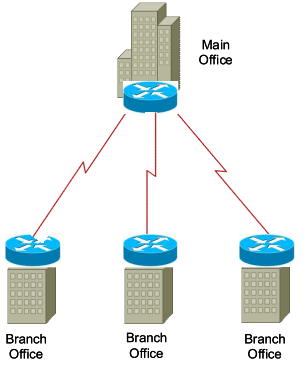
\includegraphics[scale=1]{figures/ex/cmo.png}
\caption{Connection to the Main Office}
\end{figure}

"\`E stata progettata una rete di una piccola compagnia con una topologia gerarchica \textit{Hub-And-Spoke}. La LAN in ogni ufficio secondario è connessa all'ufficio principale tramite un router ed un link con capacità $C = 128\ Kbps$. Dove $(1\ Kbit = 1000\ bits)$. In uno dei siti il flusso del traffico in uscita è generato principalmente da applicazioni CAD fino ad adesso. Per quel traffico, che può essere modellato come un processo di Poisson con rate $\lambda_0 = 3\ pkt/s$, è richiesto che il queueing delay nel router (per i pacchetti in coda) sia meno di $0.5$ secondi con probabilità più grande di $0.99$. A seguito di una nuova configurazione dei processi di business, è anche necessario installare un numero di computer per l'automazione degi uffici. Ci si aspetta che ognuno di loro generi un flusso di pacchetti verso l'ufficio centrale ad un average rate di $\lambda = 1\ pkt/s$. Per quest'ultimo flusso, è richiesto che l'average time speso nel router sia minore od uguale ad 1s.

Le dimensioni dei pacchetti possono essere modellate da variabili casuali indipendenti che sono esponenzialmente distribuite con valore medio $D = 500bytes$.

\begin{itemize}
\item Si assuma che la coda di output del router abbia capacità infinita e sia condivisa da tutti i flussi di traffico secondo disciplina di coda FCFS. Si determini il massimo numero $M$ di nuovi computer che possono essere installati;
\item Considerando il valore $M$, si valuti la \textit{packet loss probability} nel caso la dimensione della coda di output sia limitata a 10 pacchetti.
\end{itemize}

Abbiamo una topologia Hub-And-Spoke. (centro-e-raggi, topologia stellare). $C = 128\ Kbps$. Dove $(1\ Kbit = 1000\ bits) \implies C = 128000\ bit/s$. $\lambda_o = 3\ pkt/s\ \land\ \lambda = 1\ pkt/s$. Si richiede che il ritardo di accodamento nel router sia minore di $0.5s$ con probabilità maggiore di $0.99$. Le lunghezze dei pacchetti sono distribuite esponenzialmente di media 500 bytes. Politica FCFS. Quanto è il numero massimo di computer installabili $M$?

Supponiamo di indicare con $W$ la v.a. che rappresenta il ritardo di accodamento; il vincolo è il seguente, con $(\tau = 0.5s),\ \underline{s=threshold}=0.99$:

\[
	\Pr\{W < (\tau = 0.5s)\ |\ si\ faccia\ coda\} > (0.99 = s)
\]

Indichiamo con $\bar{R}$ il ritardo di accodamento per l'ultimo flusso. Deve valere: $\bar{R} \leq 1s$. Cerchiamo di risolvere il sistema con M/M/1. Abbiamo già delle ipotesi, ma dovremo farne di aggiuntive. Modelliamo quindi il router con un sistema a coda M/M/1:

Abbiamo un buffer output, ed un trasmettitore collegato in serie che è associato al link di uscita. Ipotesi: flusso secondo il quale arrivano i pacchetti di POISSON (pacchetti applicazioni CAD). Stiamo trascurando il ritardo di elaborazione router.
Capacità di elaborazione talmente elevata da ritenersi trascurabile (NO BOTTLENECK). Inoltre: $(d = +\infty)$. Il router opera con FCFS (quella contemplata dal sistema a coda M/M/1). Ipotesi aggiuntiva: certo numero di flussi, $M$ riguardanti i computer dell'Office Automation. Processo degli arrivi di POISSON. Ipotesi di indipendenza abbastanza scontata, dal momento che i vari utenti non si influenzeranno a vicenda. $M\lambda$. Ipotesi aggiuntiva: supponiamo che gli arrivi dei pacchetti relativi ai computer Office Automation siano indipendenti da quelli delle applicazioni CAD. Effettuando il POOLING, abbiamo che la distribuzione risultante è sempre un processo di POISSON con parametro dato dalla somma dei parametri: $\lambda' = \lambda_0+M\lambda$. Quindi $\lambda'$ è la velocità di arrivo dei clienti nel sistema a coda, $\mu$ è la velocità di servizio del router, ovvero il numero medio di pacchetti elaborati dal router per unità di tempo quando il router è costantemente occupato. Abbiamo dei tempi di servizio indipendenti, identicamente distribuiti ed indipendenti dai tempi di interarrivo. Nel sistema i tempi di servizio corrispondono ai tempi di trasmissione. Questo tempo di servizio è legato al parametro (valore medio) $D$ della distribuzione esponenziale che caratterizza la lunghezza dei pacchetti. Quindi abbiamo che il tempo medio di trasmissione è $\frac{1}{\mu} = \frac{D}{C} [s]$, ed abbiamo quindi $\mu = \frac{C}{D} = \frac{1}{D/C} = 32\  [pkt/s]$, ovvero abbiamo 32 pacchetti in media quando il router è costantemente occupato.

\begin{itemize}

\item{\textbf{Parte 1}}

Tutte le ipotesi del sistema a coda M/M/1 sono rispettate. Possiamo quindi utilizzarne i risultati: $\{\lambda',\mu\}$. Dobbiamo andare ad imporre quelle due condizioni. Per un M/M/1, il ritardo per cliente è $\bar{R} = \frac{1}{(\mu-\lambda)}$. Il ritardo per cliente è una v.a. distribuita esponenzialmente $\iff [R \sim EXP(\mu-\lambda)]$. Guardando adesso all'altra condizione, si dimostra che:

\[
	[F_W(y) = \Pr\{W \leq y\} = 1-\rho\e^{-\mu(1-\rho)y},\ y\geq 0]
\]

Tale è la CDF del Ritardo del cliente nella CODA! (Nella sola coda). $W$ sarebbe il tempo di permanenza del cliente nella SOLA coda del sistema a coda M/M/1. Distribuzione valutata su tutti i clienti (anche per quelli che non ci interessano). Dobbiamo condizionarla al fatto che si faccia coda. Quando $(y=0)$, esce $\Pr\{W\leq 0\} = (1-\rho)$. Ovvero la probabilità che il tempo di permanenza in fila di attesa sia nullo è pari a $(1-\rho)$. $\Pr\{W = 0\} = 1-\rho$. Si tratta di una v.a. mista. $\rho$ è il fattore di utilizzazione del router. Nel sistema a coda M/M/1, $\rho = (\frac{\lambda'}{\mu})$. Nell'M/M/1, $(1-\rho)=\pi_0^{(a)}$, ovvero la frazione di tempo a regime nel quale nel sistema a coda non vi sono clienti. La probabilità che il tempo di permanenza sia nullo è PARI alla probabilità che all'arrivo la fila di attesa SIA VUOTA!

\[
	[\Pr\{W = 0\} = 1-\rho = \pi_0]
\]

Questa è pari alla probabilità che un cliente AL SUO ARRIVO vada subito al router. In generale: $\pi_i^{(a)} \neq \pi_i$, laddove il primo membro della disuguaglianza riflette la visione dei clienti all'arrivo, valutata solo sugli istanti di arrivo, mentre il secondo membro riflette la visione all'esterno del sistema, considerando tutto l'asse temporale. $\pi_i$, ponendo l'ERGODICIT\`A, rappresenta la frazione di tempo nel quale vi sono $i$ clienti a regime. Mentre $\pi_i^{(a)}$ è la probabilità calcolata valutando SOLTANTO GLI ISTANTI DI ARRIVO! Frazione degli ARRIVI che trovano il sistema (a regime) nello stato $i$. Infatti potremmo avere ad esempio: $\{\{\pi_1 = \frac{1}{3},\ \pi_0=\frac{2}{3}\}\ \land\ \{\pi_0^{(0)}=1,\ \pi_1^{(0)}=0,\ \pi_2^{(0)}=0\}\}$.

\begin{thrm}{\textbf{P.A.S.T.A. \textit{POISSON ARRIVALS SEE TIME AVERAGES}}}

\[
	\left\{
	\begin{aligned}
	&\pi_i = \lim_{t\to\infty}{\Pr\{N(t)=i\}}\\
	&\pi_i^{(a)} = \lim_{t\to\infty}{\Pr\{N(t)=i\ |\ un\ arrivo\ subito\ dopo\ t\}}
	\end{aligned}
	\right.
\]

Se gli arrivi dei clienti si susseguono con processo di POISSON, abbiamo che: $\pi_i^{(a)}=\pi_i,\ \bar{N}=\sum_{i=0}^\infty{i\pi_i}$

\end{thrm}

Dove la prima equazione è una quantità calcolata sull'insieme delle realizzazioni. (Media di insiemi). Ma se vale L'ERGODICIT\`A, allora le medie d'insieme coincidono con le medie TEMPORALI. $\pi_i$ rappresenta la frazione del tempo nella quale vi sono a regime $i$ clienti nel sistema; $\pi_i^{(a)}$ rappresenta la frazione dei clienti che, all'arrivo trovano il sistema nello stato $i$. Coincide con la probabilità (a regime), che all'arrivo un cliente trovi $i$ clienti nel sistema. Rappresenta cosa vedono i clienti all'arrivo.

Per i nostri scopi, $[\pi_0^{(a)} = \Pr\{W = 0\}] = [\underline{1-\rho = \pi_0}]$, ove la parte sottolineata è la probabilità che vi siano 0 clienti, in un istante qualsiasi, mentre il primo membro è la probabilità che un cliente, al suo arrivo, trovi 0 clienti nel sistema. Grazie al teorema appena visto, esse coincidono. 

$\rho$ è la frazione del tempo in cui il router è occupato $\implies$ probabilità che il router sia occupato. $(1-\rho)$ è la probabilità che il router sia quindi libero. 
$\Pr\{W \leq \tau\ |\ si\ fa\ coda\} = (\dots)$ è la probabilità che il tempo di permanenza in FILA DI ATTESA sia inferiore (od uguale) a $\tau$, quando si fa coda.
Quindi abbiamo:

\[
	(\dots) = 1-\Pr\{W > \tau\ |\ si\ fa\ coda\} = 1-\frac{\Pr\{W > (y := \tau),\ si\ fa\ coda\}}{\Pr\{si\ faccia\ coda\}} = (\dots)
\]

Notiamo che $\{W > y\} \supseteq \{si\ fa\ coda\}$, ed inoltre, dal teorema appena visto (PASTA) vale che: $1-\pi_0^{(a)} = 1-\pi_0 = \rho = \Pr\{si\ fa\ coda\}$, ovvero la probabilità che all'arrivo di un cliente il servitore sia occupato coincide con la probabilità di fare coda. Ciò implica: $\implies$

\[
	(\dots) = 1-\frac{\Pr\{W>\tau\,\ si\ fa\ coda\}}{\Pr\{si\ fa\ coda\}} = 1-\frac{\Pr\{W\geq\tau\}}{\rho} =
\]
\[
	= 1-\frac{\rho\e^{-\mu(1-\frac{\lambda}{\mu})y}}{\rho} = 1-\e^{-\mu(1-\frac{\lambda}{\mu})y},\ y\geq 0
\]

Concludiamo che:

\[
	\Pr\{W \leq y\ |\ si\ fa\ coda\} = 1-\e^{-\mu(1-\frac{\lambda}{\mu})y} \iff W|_{\{si\ fa\ coda\}} \sim EXP(\mu-\lambda)
\]

quindi nell'M/M/1, $R=W|_{\underline{\{si\ fa\ coda\}}}$. Si riferisce proprio alla medesima distribuzione esponenziale, con il medesimo parametro!

Consci che $[R = \frac{1}{\mu-\lambda'}]$, allora procediamo:

\[	
	1-\e^{-(\mu-\lambda')\tau} > s \implies \e^{-(\mu-\lambda')\tau} < (1-s) \implies -(\mu-\lambda')\tau < \log(1-s) \implies (\dots)
\]
\[
	(\dots) \implies -\mu\tau +\lambda'\tau < \log(1-s) \implies [\lambda'\tau < \log(1-s)+\mu\tau] \implies (\dots)
\]
\[
	(\dots) \implies \lambda_0+M\lambda < \frac{\log(1-s)}{\tau} + \mu \implies M\lambda < \mu + \frac{\log(1-s)}{\tau}-\lambda_0 \implies (\dots)
\]
\[
	(\dots) \implies M < \frac{1}{\lambda}[\mu+\frac{1}{\tau}\log(1-s)-\lambda_0] = [32.8]
\]

ove il valore si è ottenuto appositamente sostituendovi i dati al secondo membro dell'ultima disequazione.

Quindi $\floor{M} = M_{max} = 32$ computer massimi.
Si ottiene $M \leq 32.8$, quindi possiamo installare MASSIMO 32 COMPUTER. D'altro canto dobbiamo rispettare anche il vincolo sull'average router time:

\[
	\bar{R} = \frac{1}{\mu-\lambda'} \implies \frac{1}{\mu-\lambda'} \leq 1s \implies ((\mu-\lambda')>0) \geq 1s \implies (\dots)
\]

ove l'ultima parentesizzazione maggiore di 0 indica la condizione di STABILIT\`A, che naturalmente deve essere sempre rispettata.

\[
	(\dots) \implies \mu - (\lambda_0+M\lambda)\geq 1 \implies \mu-\lambda_0 -M\lambda \geq 1 \implies M\leq\frac{\mu-\lambda_0-1}{\lambda} =
\]
\[
	= \frac{1}{\lambda}[\mu-\lambda_0-1] \implies M\leq 28
\]

Ne si conclude che $M_{max}=\min{\{28,32\}} = 28$ computer. Quindi: $\underline{\underline{[M\leq M_{max}=28]}}$.


\newpage

\item{\textbf{Parte 2}}: 

\subsubsection{M/M/1/k}

Consideriamo che $d = 10\ pkt$ (10 pacchetti), $d<+\infty$ ed abbiamo quindi un buffer di dimensione finita. $\iff (d=10)<+\infty$. In questo caso NON possiamo studiare il sistema con un modello M/M/1! Ci serve invece un \textit{M/M/1/k}, nel quale la dimensione del buffer è limitata. Pensiamo a $k$ come la capacità di tutto il sistema (includendo il centro di servizio). Stiamo quindi considerando un sistema a CODA CON PERDITA. Quando un elemento arrivando trova la coda piena, il sistema interviene con il meccanismo di DISCARD (avviene il fenomeno \textit{packet loss}). In questo caso $\lambda'$ è la velocità di arrivo dei clienti al sistema (POISSON). $\lambda_s$ sarà sempre la velocità di ingresso alla coda e di uscita (numero medio di clienti). $\rho=\frac{\lambda_s}{\mu}$ è il fattore di utilizzazione del servitore. Abbiamo che:

\[
	\Pr\{perdita\} = \frac{\lambda^l}{\lambda'} = \pi_k^{(a)} = \pi_k
\]

grazie a PASTA. Disegnamo il relativo DTT della catena:

\begin{center}
\begin{tikzpicture}[->, >=stealth', auto, semithick, node distance=2cm]
\tikzstyle{every state}=[fill=white,draw=black,thick,text=black,scale=1]
\node[state]    (0)                     {$0$};
\node[state]    (1)[right of=0]   {$1$};
\node[state]    (2)[right of=1]   {$2$};
\node[state] (d) [right of=2] {\ldots};
\node[state]    (km1)[right of=d]   {$k-1$};
\node[state]    (k)[right of=km1]   {$k$};
\path
(0) edge[bend left]     node{$\lambda'$}         (1)
(1) edge[bend left]     node{$\lambda'$}         (2)
    edge[bend left,below]    node{$\mu$}            (0)
(2) edge[bend left]     node{$\lambda'$}           (d)
    edge[bend left,below]    node{$\mu$}             (1)
(d) edge[bend left]         node{$\lambda'$}   (km1)
	edge[bend left,below]   node{$\mu$}          (2)
(km1) edge[bend left]       node{$\lambda'$}  (k)
	  edge[bend left,below]   node{$\mu$}     (d)
(k)   edge[bend left,below]  node{$\mu$}          (km1);
\end{tikzpicture}
\end{center}

Sia $N(t)$ il numero di clienti nel sistema a tempo $t$. 
$\Pr\{\phi_i(t) > \tau\} = (\dots)$, dove $\phi_i(t)$ indica il tempo di soggiorno residuo nello stato $i$ al tempo $t$, indica la probabilità che per almeno $\tau$ unità di tempo non ci sia alcun arrivo e NON vi sia la fine del servizio in corso, condizionata con il fatto che attualmente vi sono $i$ clienti nel sistema.

Indichiamo con $\xi_{Rt} \sim EXP(\lambda')$ la v.a. tempo di interarrivo residuo al tempo $t$, e con $\eta_{Rt} \sim EXP(\mu)$ la v.a. tempo di servizio residuo al tempo $t$. Tutte indipendenti ed indipendenti tra di loro, grazie all'ipotesi di (inter)-indipendenza. 

\[
	(\dots) = \Pr\{\xi_{Rt}>\tau,\ \eta_{Rt}>\tau\} = \Pr\{\xi_{Rt}>\tau\}\Pr\{\eta_{Rt}>\tau\} = \e^{-\lambda'\tau}\e^{-\mu\tau} = \e^{-(\lambda'+\mu)\tau}
\]

Quindi abbiamo di nuovo: $-q_{ii} = \mu+\lambda' \implies$

\[
	\tau_{i,i+1} = \frac{q_{i,i+1}}{-q_{ii}} = \frac{q_{i,i+1}}{(\mu+\lambda')}
\]

$\tau_{i,i+1}$ è la probabilità che lasciando lo stato $i$, il processo vada verso $i+1$. Sfruttando il teorema delle probabilità totali nel continuo, abbiamo: $q_{i,i+1} = (\mu+\lambda') \frac{\lambda'}{(\mu+\lambda')} = \lambda'$. Quindi sarà $\lambda'$ fino a $k-1$. La CMTC è una catena omogenea, IRRIDUCIBILE e dal momento che $\cardinality{stati}<+\infty \implies$ allora essa è SICURAMENTE ERGODICA! CATENA SEMPRE ERGODICA. Sistema STABILE.

\[
	\left\{
	\begin{aligned}
	&[\pi_i = \pi_0(\frac{\lambda'}{\mu})^i]\\
	&[\pi_0 = \frac{1}{1+\sum_{i=1}^k{(\frac{\lambda'}{\mu})^i}}]
	\end{aligned}
	\right.
\]

$i=1,2,\ \dots,\ k$.

Notiamo che:

\[
	\sum_{i=0}^k{\rho^i} = \left\{
	\begin{aligned}
	&k+1,\ \rho=1\\
	&\frac{1-\rho^{k+1}}{(1-\rho)},\ p\neq 1
	\end{aligned}
	\right.
\]

Quindi nel nostro caso abbiamo:

\[
	\pi_0 = \frac{1}{\sum_{i=0}^k{\rho^i}} = \frac{1}{\frac{1-\rho^{k+1}}{(1-\rho)}} = \frac{1-\rho}{1-\rho^{k+1}}
\]

Quindi abbiamo come Distribuzione di regime:

\[
	\pi_i = \frac{1-\rho}{1-\rho^{k+1}} \rho^i,\ i=0,1,2,\ \dots,\ k
\]

Si noti che vale anche per $i=0$. Allora:

\[
	[\Pr\{perdita\} = \underline{\pi_k^{(a)} \stackrel{PASTA}{=} \pi_k} = [\frac{1-\rho}{1-\rho^{k+1}} \rho^k]]
\]

da valutarsi con $k=10+1=d+1<+\infty$, in quanto include anche il centro di servizio.
Facendo i calcoli esce $0.07 \implies (70\%)$.

La probabilità di perdita si poteva trovare, come precedentemente enunciato, anche effettuando il rapporto $\frac{\lambda_L}{\lambda'}$. Banalmente, per SPLITTING si ha: $[\lambda_L=\lambda'-\lambda_S]$. Le perdite comunque mi fanno venire meno la caratteristica di POISSON.

\[
	\Pr\{k\ arrivi\ in\ \tau\} = \frac{(\lambda\tau)^k}{k!}\e^{-\lambda\tau}
\]

ma la sequenza degli ingressi a valle della diramazione NON è più di POISSON! $\rho = (\frac{\lambda_S}{\mu})$ rappresenta il fattore di utilizzazione, quindi la frazione del tempo a regime in cui il servitore è occupato. $\rho=1-\pi_0 \implies \pi_0=1-\rho$.

$\lambda_S=\mu(1-\pi_0)$ rappresenta la velocità delle partenze (\textit{departure}) dei clienti dal mio sistema. Abbiamo: $[\pi_0 = \frac{1-\rho}{1-\rho^{k+1}}]$.

\[
	\lambda_L = \lambda'-\lambda_S = \lambda'-\mu(1-\pi_0)
\]

Quindi $\lambda_S$ è la velocità secondo la quale i clienti partono dal sistema, od anche la media dei clienti che partono all'unità di tempo. Guardando il DTT, vi è una partenza quando FINISCE un servizio! Determinando le frequenze delle transizioni a sinistra, potremo sapere le frequenza delle partenze. La frequenza delle partenze si ottiene sommando tutte le frequenze delle transizioni $\pi_iq_{ij}$, sfruttando opportunamente l'inversa della CONDIZIONE DI \underline{NORMALIZZAZIONE}:

\[
	\pi_1\mu + \pi_2\mu +\ (\dots)\ +\pi_k\mu = \mu\sum{\pi_i} = [\lambda_S = \mu(1-\pi_0)]
\]

Stessa cosa mettendoci a valle della diramazione ed a monte della coda: (ARRIVI DI CLIENTI dall'esterno del sistema). $\lambda_S$ rappresenta qui il numero medio di clienti che entrano nel sistema per unità di tempo.

\[
	\lambda_S = [\pi_0\lambda'+\pi_1\lambda'+\ \dots\ +\pi_{k-1}\lambda'] = \lambda'
\]

Valgono le equazioni di bilanciamento locale, valide solo per una CMTC di nascita e morte (BDCMTC):

\[
	\pi_1\mu = \pi_0\lambda' \implies \pi_{k+1}\mu = \pi_k\lambda'
\]

ovvero le sommatorie sono identiche.

$\frac{\lambda_L}{\lambda'}$ rappresenta la probabilità di perdita.

\begin{thrm}{\textbf{Probabilità di perdita}}

\[
	\Pr\{perdita\} = \frac{1-\rho}{1-\rho^{k+1}}\rho^k = \pi_k^{(a)} = \pi_k
\]

ove $\pi_k$ rappresenta la probabilità che il sistema si trovi nello stato $k$ in un istante qualsiasi. Abbiamo anche:

\[
	\Pr\{perdita\} = \frac{(\lambda_L = \lambda'-\lambda_S)}{\lambda'} = 1-\frac{\lambda_S}{\lambda'} = (\dots)
\]
\end{thrm}

Ove $\lambda_S$ è stato trovato applicando Little al primo sottosistema, ottenendo quindi $\lambda_S =\mu(1-\pi_0)$.

\begin{proof}

\[
	(\dots) = 1-\frac{\mu(1-\pi_0)}{\lambda'} = 1-\frac{1}{\rho}(1-\frac{1-\rho}{1-\rho^{k+1}}) = 1-\frac{1}{\rho}(\frac{1-\rho^{k+1}-1+\rho}{1-\rho^{k+1}})
\]
\[
	1-\frac{1}{\rho}\rho \frac{(1-\rho^k)}{(1-\rho^{k+1})} = \frac{1-\rho^{k+1}-1+\rho^k}{1-\rho^{k+1}} = \frac{\rho^k(1-\rho)}{(1-\rho^{k+1})};
\]

\end{proof}

La probabilità di perdita di un cliente deve quindi alla fine coincidere con il rapporto $\frac{\lambda_L}{\lambda'}$.

\end{itemize}

\subsection{Sistemi a coda M/M/m}

Il sistema a coda M/M/m rappresenta una generalizzazione del sistema M/M/1. Abbiamo $m$ router.
Anche in questo caso, il processo degli arrivi è un processo di POISSON con velocità $\lambda$. ($\lambda$ = velocità di arrivo dei clienti). In media arrivano $\lambda$ clienti per unità di tempo. Anche in questo caso i tempi di servizio sono v.a. indipendenti (mutuamente), i.d. con una distribuzione esponenziale negativa unilatera, con tempo medio di servizio $(\frac{1}{\mu})$, ed indipendenti statisticamente dai tempi di interarrivo dei clienti nel sistema a coda. La velocità del centro di servizio sarà variabile (il centro di servizio include ora $m$ servitori), ovvero dipende dal numero di router attivi in un certo istante di tempo. Se $i$ è il numero di clienti nel sistema a coda in un certo istante di tempo, $i<m \implies i\mu$ velocità del centro di servizio. $i$ sono i clienti IN TUTTO IL SISTEMA! In totale quindi i servitori attivi serviranno $i\mu$ utenti $\forall$ unità di tempo. $i\geq m$ tutti gli $m$ servitori saranno attivi $\implies$ velocità $m\mu$. Quindi $i\geq m$ centro di servizio alla massima velocità possibile. $m\mu$ = capacità TOTALE DI SERVIZIO DEL SISTEMA (del centro di servizio). Come nella M/M/1, la dimensione del buffer e la popolazione sono illimitate ($\iff d,e<+\infty$). Disciplina di queueing di default (FCFS). Modellabile come uno stack FIFO. Se arriva un cliente e c'è un certo numero di router liberi, sarà assegnato in maniera random ad uno di questo. Approccio MARKOVIANO basato sul processo stocastico che si riferisce al numero di clienti nell'intero sistema a coda al tempo $t$, ovvero $N(t)$. La sua evoluzione sarà determinata dalle v.a. tempi di interarrivo e tempi di servizio. Dato che per queste ipotesi queste v.a. sono prive di memoria e statisticamente indipendenti $\implies$ siamo dinanzi una CMTC, il cui diagramma dei tassi di transizione è il seguente:

\begin{center}
\begin{tikzpicture}[->, >=stealth', auto, semithick, node distance=2cm]
\tikzstyle{every state}=[fill=white,draw=black,thick,text=black,scale=0.8]
\node[state]    (0)                     {$0$};
\node[state]    (1)[right of=0]   {$1$};
\node[state]    (2)[right of=1]   {$2$};
\node[state] (d) [right of=2] {\ldots};
\node[state]    (mm1)[right of=d]   {$m-1$};
\node[state]    (m)[right of=mm1]   {$m$};
\node[state]    (mp1)[right of=m]   {$m+1$};
\node[state]    (mp2)[right of=mp1]   {$m+2$};
\node[state]    (d2)[right of=mp2]  {\ldots};

\path
(0) edge[bend left]     node{$\lambda$}         (1)
(1) edge[bend left]     node{$\lambda$}         (2)
    edge[bend left,below]    node{$\mu$}            (0)
(2) edge[bend left]     node{$\lambda$}           (d)
    edge[bend left,below]    node{$2\mu$}             (1)
(d) edge[bend left]         node{$\lambda$}   (mm1)
	edge[bend left,below]   node{$3\mu$}          (2)
(mm1) edge[bend left]       node{$\lambda$}  (m)
	  edge[bend left,below]   node{$(m-1)\mu$}     (d)
(m)   edge[bend left]   node{$\lambda$}      (mp1)
      edge[bend left,below]  node{$m\mu$}          (mm1)
(mp1) edge[bend left]       node{$\lambda$}  (mp2)
	 edge[bend left,below]   node{$m\mu$}      (m)
(mp2) edge[bend left]       node{$\lambda$}   (d2)
      edge[bend left,below] node{$m\mu$}    (mp1)
(d2) edge[bend left,below]   node{$m\mu$}     (mp2);
\end{tikzpicture}
\end{center}

CMTC nascita e morte (BDCMTC), con $\cardinality{stati}=+\infty$ (infiniti), fila di attesa di dimensione illimitata. Tassi di nascita pari a $\lambda$, tassi di morte $m\mu$, che sarebbe il tasso di morte nello stato $i$ prima che si saturino i servitori disponibili, dopodiché $(i\geq m)$, sempre pari a $m\mu$.

\subsubsection{Calcolo dei tassi (velocità) di transizione}

Supponiamo $N(t)=i\neq 0$ ($i$ clienti nel mio intero sistema a coda), ovvero qualsiasi stato diverso dallo stato banale. Il successivo cambiamento di stato sarà legato od all'arrivo di un nuovo cliente od al completamento di uno dei servizi eseguiti in parallelo al tempo $t$. Comunque abbiamo $i$ clienti totali. Possibili casi: $\{i++,\ i--\}$. L'intervallo di tempo da $t$ al successivo arrivo lo indichiamo con $\underline{\xi_R(t) \sim EXP(\lambda)}$, ovvero il tempo di interarrivo residuo (stessa caratteristiche dei tempi di interarrivo). Il tempo che passa tra l'istante presente $t$ ed il successivo completamento del servizio, sarà $\eta_R(t)$, e sarà pari al minimo dei tempi di servizio residui in $t$. Ci saranno un certo numero di servizi. $\eta_R(t) = \min{\{...\}}$, ovvero al minimo dei tempi di servizio residui legati a quei servizi che al tempo $t$ stanno procedendo in parallelo. Quando $i<m$, ci saranno $i$ servizi che stanno procedendo in parallelo. Anche i tempi di servizio residui sono \underline{indipendenti} fra di loro per ipotesi, dal momento che i servizi procedono in parallelo senza influirsi. Quindi $\eta_R(t) \sim EXP(\sum_i{\mu_i})$. Quando $i<m\implies$ $\eta_R(t) \sim EXP(i\mu)$. Se invece $i\geq m$, $\eta_R(t) \sim EXP(m\mu)$. A questo punto, il tempo che passa dall'istante presente $t$ e la successiva transizione di stato, sarà $\phi_i(t)$ (tempo di soggiorno residuo nello stato $i$ al tempo $t$) prima di cambiare stato $\implies$

\[
	\phi_i(t) = \min{\{\xi_R(t),\ \eta_R(t)\}} \implies \phi_i(t) \sim EXP(-q_{ii})
\]

ove l'ultima implicazione è valida grazie al fatto che queste variabili casuali sono i.i.d. ed indipendenti tra di loro. Abbiamo:

\[
	-q_{ii} = \left\{
	\begin{aligned}
	&(\lambda+i\mu),\ i<m\\
	&(\lambda+m\mu),\ i\geq m
	\end{aligned}
	\right.
\]

(Velocità totale di uscita \underline{dallo stato i}). Parametro $-q_{ii}$. Quindi, quella quantità rappresenta con che velocità in totale esco dallo stato. Ma se $\underline{i<m}$, perché $q_{i,i+1} = \lambda,\ q_{i,i-1}=i\mu$. Solito giochetto. (Se $i\geq m,\ q_{i,i-1}=m\mu$). Consideriamo:

\[
	\tau_{i,i+1} = \frac{q_{i,i+1}}{-q_{ii}} = \Pr\{\xi_R(t) < \eta_R(t)\} = (\dots)
\]

ove l'ultima quantità rappresenta la probabilità che il prossimo arrivo preceda la fine del servizio (il completamento del servizio). Dobbiamo quindi applicare il teorema delle probabilità totali nel continuo, ottenendo alla fine:

\[
	(\dots) = \left\{
	\begin{aligned}
	&\frac{\lambda}{\lambda+i\mu},\ i<m\\
	&\frac{\lambda}{\lambda+m\mu},\ i\geq m
	\end{aligned}
	\right.
\]

CMTC OMOGENEA, IRRIDUCIBILE, ma non sappiamo tuttavia se è ERGODICA.

\[
	\left\{
	\begin{aligned}
	&[\pi_0 = \frac{1}{1+\sum_{i=1}^{m-1}{(\frac{\lambda}{\mu})^i\frac{1}{i!}} + (\frac{m^m}{m!})\sum_{i=m}^\infty{(\frac{\lambda}{m\mu})^i}}]\\
	&\left\{
	\begin{aligned}
	&\pi_i = \pi_0 (\frac{\lambda}{\mu})^i \frac{1}{i!},\ i<m\\
	&\pi_i = \pi_0 (\frac{\lambda}{\mu})^i \frac{1}{m!m^{i-m}},\ i\geq m
	\end{aligned}
	\right.
	\end{aligned}
	\right.
\]

Dobbiamo capire qual'è la CONDIZIONE MAX di ERGODICIT\`A (si ha una condizione di regime). La sommatoria ad infiniti termini (serie) a denominatore di $\pi_0$ deve convergere di nuovo. La condizione di ERGODICIT\`A è quindi: $(\frac{\lambda}{m\mu}) < 1$ (convergenza della serie geometrica). Quando $\rho := \frac{\lambda}{m\mu} < 1$ questa sommatoria (serie) converge, e si ha una distribuzione che è quella di regime. $[\lambda < m\mu]$ è proprio la condizione di STABILIT\`A, la quale indica che la velocità di arrivo deve essere minore della capacità totale di servizio. Serve sostanzialmente per evitare l'"ingolfamento". $\rho$ è il fattore di utilizzazione del generico router (Non del centro di servizio). Ognuno dei router avrà un fattore di utilizzazione pari a $\rho$, quando il carico è EQUAMENTE DISTRIBUITO. $\frac{\lambda}{m}$ sarà la capacità di arrivo del singolo cliente. Servono in media lo stesso numero di clienti $\forall$ unità di tempo. Tutti lavoreranno alla stessa maniera. Ogni router si vedrà arrivare quindi $\frac{\lambda}{m}$ clienti per unità di tempo. Fattore di utilizzazione; frazione di tempo quando il servitore è occupato. Infatti, applicando \underline{Little} troviamo: $(\frac{\lambda}{m})(\frac{1}{\mu})$, trovando la frazione di tempo nel quale il router è occupato per unità di tempo nella quale il router è costantemente occupato, quando il carico di lavoro è EQUAMENTE DISTRIBUITO. $\frac{\lambda}{\mu}$ è l'\textit{intensità di traffico} (arrivano $\lambda$ clienti, $\frac{1}{\mu}$ è il lavoro medio richiesto dal cliente). Quindi sfruttiamo ancora Little e troviamo: $\lambda(\frac{1}{\mu})$, trovando così il \underline{\underline{CARICO MEDIO DI LAVORO}}. 

\[	
	[\frac{\lambda}{\mu} = m(\rho := \frac{\lambda}{m\mu}) = m\rho]
\]

Si usi questo fatto per vedere a cosa converge la sommatoria geometrica:

\[	
	[\pi_0 = \frac{1}{\sum_{i=0}^{m-1}{(m\rho)^i \frac{1}{i!}} + (\frac{m^m}{m!} \frac{\rho^m}{1-\rho} = \frac{(m\rho)^m}{m!(1-\rho)})}]
\]

e tramite questa espressione possiamo ovviamente trovare le $\pi_i$.

ERGODICIT\`A se: $[\underline{\lambda < m\mu}]$. Abbiamo trovato la distribuzione di regime. Nel caso M/M/1, abbiamo poi ricavato tutti i numeri medi di clienti e tempi di servizio, etc. Nel caso M/M/1 siamo partiti da $\bar{N}$.

\subsubsection{Quantità medie tipiche}

Adesso partiamo da $\bar{T}$, ovvero il ritardo medio per cliente a regime. Terminologia tempo di risposta. $\bar{T}$ tempo di risposta. Tempo di permanenza del cliente nel sistema a coda. Abbiamo:

\[
	(\bar{T} := \E[T]) = \E[t_s] + \E[W] = \frac{1}{\mu} + (\dots)
\]

ove $W$ è il tempo di accodamento, ovvero il queueing delay. Adesso per valutare il tempo medio di permanenza in fila di attesa utilizziamo il concetto di \textit{MEDIA CONDIZIONATA}:

\[
	(\dots) = \E[\E[W\ |\ k\ clienti\ all'arrivo]] = \mathord{\cdot}(k)
\]

dove $\{k\ clienti\ all'arrivo\}$ sarebbe l'evento nel quale troviamo $k$ clienti all'arrivo in testa al sistema. Tempo di permanenza, sapendo che all'arrivo il cliente trova $k$ clienti nel sistema. Quindi:

\[
	\bar{T} = \frac{1}{\mu} + \sum_{k=m}^\infty{\E[W\ |\ k\ clienti\ all'arrivo]}\pi_k^{(a)}
\]

Notiamo che $k$ parte da $m$, perché se $k<m$ quella quantità sarebbe nulla!
Il tempo medio di permanenza nella fila di attesa è nullo quindi se $k<m$! Se arrivato nel sistema a coda trovo un numero $(k<m)$ di clienti, allora VADO DIRETTAMENTE nel CENTRO DI SERVIZIO! Sommatoria che parte da $m$ quindi. Volendo la si potrebbe fare partire da 0, senza alcuna perdità di generalità, dal momento che i primi $(m-1)$ termini sarebbero comunque nulli. Abbiamo:

\[	
	\bar{T} = \frac{1}{\mu} + \sum_{k=m}^\infty{\frac{k-m+1}{m\mu}(\pi_k^{(a)}=\pi_k)} = (\dots)
\]

Dove l'uguaglianza tra parentesi deriva da PASTA. Abbiamo sfruttato il fatto che: $[\E[W|k] = \frac{k-m+1}{m\mu}]$. Siamo nel caso $k\geq m$, ove vi sono $m$ clienti al servizio, $(k-m)$ clienti in fila di attesa ed io. Dopo che vi sarà il completamento di $(k-m)$ servizi mi troverò in testa alla fila di attesa. Ma dovrò quindi attendere il completamento di un ulteriore servizio (ecco perché il termine $+1$). Ma il tempo tra il completamento del servizio corrente ed il successivo è $(\frac{1}{m\mu})$! ($\leftarrow$ tempo medio di servizio). $\implies$

\[
	(\dots) = \frac{1}{\mu} + \sum_{k=m}^\infty{(\frac{k-m+1}{m\mu})\pi_0\frac{m^m}{m!}\rho^k} = \frac{1}{\mu} + \pi_0\frac{m^m}{m!}\sum_{k=m}^\infty{\frac{k-m+1}{m\mu}\rho^k} = (\dots)
\]

A questo punto possiamo porre: $i := k-m+1$, ed otteniamo:

\[
	(\dots) = \frac{1}{\mu} + \pi_0\frac{m^m}{m!m\mu}\sum_{i=1}^\infty{i(\rho^{i-1+m} = \rho^{i-1}\rho^m)} =
\]
\[
	= \frac{1}{\mu} + \frac{(m\rho)^m}{m!m\mu}\pi_0\sum_{i=1}^\infty{i\rho^{i-1}} = [\frac{1}{\mu} + \frac{\pi_0(m\rho)^m}{m!m\mu} \frac{1}{(1-\rho)^2}]
\]

Abbiamo quindi trovato il RITARDO MEDIO PER CLIENTE. Volendo potremmo anche trovare con Little: $\bar{N}=\lambda\bar{T} = (\dots)$. Spesso in letteratura si esprime $\bar{T}$ in funzione della probabilità di attesa:

\[
	\Pr\{accodamento\ (queueing)\} = \sum_{k=m}^\infty{(\pi_k^{(a)}=\pi_k)}
\]

sarebbe ovvero la sommatoria di queste probabilità. Si deriva quindi la \textit{C di ERLANG}. (La B di ERLANG è invece collegata alla probabilità di perdita (M/M/m/0)). 

Siamo in un sistema a coda M/M/m. Ritardo medio per cliente:

\[
	\left\{
	\begin{aligned}
	&\bar{T} = \frac{1}{\mu} + \frac{\pi_0(m\rho)^m}{m!m\mu} \frac{1}{(1-\rho)^2}\\
	&\rho = \frac{\lambda}{m\mu},\ \rho<1
	\end{aligned}
	\right.
\]

ove l'ultima equazione del sistema indica la condizione di \underline{STABILIT\`A}. Questa quantità ($\bar{T}$), viene solitamente espressa in letteratura in funzione della probabilità di ATTESA, nella quale dobbiamo considerare la situazione in cui abbiamo almeno $m$ clienti nel sistema a coda quando arriva un cliente:

\[
	\Pr\{queueing\} = \sum_{k=m}^\infty{(\pi_k^{(a)}=\pi_k)} = \sum_{k=m}^\infty{\pi_k} =
\]
\[
	\sum_{k=m}^\infty{\pi_0(\frac{\lambda}{m\mu} = \rho)^k \frac{m^m}{m!}} = \pi_0\frac{m^m}{m!}\sum_{k=m}^\infty{\rho^k} = (\dots)
\]

Siamo dinanzi una sommatoria geometrica, quindi:

\[
	(\dots) = \pi_0\frac{m^m}{m!} (\frac{\rho^m}{1-\rho}) = \frac{\pi_0(m\rho)^m}{m!(1-\rho)} := C(m,\frac{\lambda}{\mu})
\]

Abbiamo ottenuto quest'espressione $C(m,(\frac{\lambda}{\mu}))$, nota come funzione \textit{C di ERLANG} con parametro: $\{m,(\frac{\lambda}{\mu})\}$. Ci sono delle tabelle per questa formula. Abbiamo ricavato un modello per la M/M/m. Possono essere utilizzate per modellare quei sistemi di servizio che prevedono diverse risorse. Sistemi di servizio con un certo numero di risorse, corrispondenti ai router $(m)$, laddove $(i\geq m \implies\ queueing)$.

Modello M/M/m. Dobbiamo però ritrovare le ipotesi dietro all'M/M/m nel mondo reale. Call-center ad esempio. Processo secondo il quale si susseguono gli arrivi al sistema a coda dev'essere ben modellabile come un processo di POISSON. Durata media delle telefonate (tempi medi di servizio) $(\frac{1}{\mu})$. In un call center mi ritrovo queste ipotesi. Ci vorrebbero anche le ipotesi sulla dimensione del buffer e della popolazione. $(d,e = +\infty)$. Dimensionamento del numero massimo di operatori (servitori) in base ad un predeterminato massimo valore da non scavalcare relativo alla probabilità di accodamento. $\{\lambda,\frac{1}{\mu}\} \to m$. Problema di progetto. Potremo anche voler affrontare un problema di ANALISI. Durata media delle telefonate $(\frac{1}{\mu})$. [ANALISI $\rightarrow$ PROGETTO]. In funzione della C di ERLANG, troviamo il valore del ritardo medio per cliente:

\[
	\bar{T} = \frac{1}{\mu} + C\frac{1}{m\mu}(\frac{1}{1-\rho}),\ \rho<1
\]

Ricordiamo che $(C\ di\ ERLANG = \Pr\{queuing\})$. Adesso, noto il valore del ritardo medio per cliente, applico Little e trovo:

\[
	\bar{N} = \lambda\bar{T} = \frac{\lambda}{\mu} + C\frac{\lambda}{m\mu}(\frac{1}{1-\rho}) = [m\rho + C\rho(\frac{1}{1-\rho})]
\]

Troviamo ora il tempo medio di permanenza nella sola fila di attesa, dove $(\rho := \frac{\lambda}{m\mu})$:

\[
	\bar{W} = \bar{T} - (T_s = \frac{1}{\mu}) = C\frac{1}{m\mu}(\frac{1}{1-\rho})
\]

E adesso il numero medio di clienti nella sola fila di attesa, $\bar{N_q}$

\[
	[\bar{N_q} = \lambda\bar{W} = C\rho(\frac{1}{1-\rho})]
\]

Dove abbiamo nuovamente applicato Little al sottosistema costituito dalla sola fila di attesa. Ora passiamo al centro di servizio, ragionando con gli stessi argomenti:

\[
	\left\{
	\begin{aligned}
	&(T_s=\frac{1}{\mu})\\
	&\bar{N_s} = m\rho := \frac{\lambda}{\mu} = \lambda(\frac{1}{\mu})
	\end{aligned}
	\right.
\]

$\rho$ è il FATTORE DI UTILIZZAZIONE. A REGIME $(\rho<1)$. Ricordiamo che $\lambda$ è sempre la velocità di arrivo.

\subsubsection{Confronto tra tre sistemi MARKOVIANI}

Questi tre sistemi MARKOVIANI hanno la stessa capacità di servizio e stessa velocità tutti tra di loro:

\begin{itemize}

\item{1)}: Un singolo sistema M/M/1 con velocità di arrivo $m\lambda$ e velocità di servizio del singolo servitore pari a $m\mu$. Parametri: $\{m\lambda,m\mu\}$;
\item{2)}: $m$ code M/M/1, ogni coda con velocità di arrivo $\lambda$ e di servizio $\mu \implies\ \{m\lambda,m\mu\}$ come parametri;
\item{3)} Sistema M/M/m con velocità di arrivo $m\lambda$ ed $m$ servitori. Ricordiamo che qui vale:

\[
	[\frac{1}{\mu} + C\frac{1}{m\mu}(\frac{1}{1-\rho}) = \bar{T},\ (\rho<1)]
\]

Abbiamo parametri: $\{m\lambda,m\mu\}$.

\end{itemize}

Tre sistemi che hanno tutti la stessa velocità di arrivo e di servizio. Confrontiamo i ritardi medi di permanenza per i clienti. Dobbiamo quindi stilare una graduatoria:
Effettuiamo un confronto:

\[
	\left\{
	\begin{aligned}
	&\bar{T_1} = \frac{1}{m\mu-m\lambda} = \frac{1}{m(\mu-\lambda)}\\
	&\bar{T_2} = \frac{1}{\mu-\lambda}\\
	&\bar{T_3} = ?
	\end{aligned}
	\right.
\]

Dovremmo fare i conti con l'espressione di $\bar{T}$ precedentemente trovata. Ma, intuitivamente la classifica sarebbe: $\{1,3,2\}$. Il primo sarebbe il migliore, sebbene poco attuabile nella pratica. Ci accontentiamo del terzo sistema. Primo sistema non attuabile come umani come router. Il primo lavora sempre alla capacità di servizio, mentre il terzo ha capacità di servizio $m\mu$ solo quando $i\geq m$!

\subsubsection{M/M/m/0}

In questo sistema abbiamo 0 come dimensione del buffer \newline
$\iff (d=0)<+\infty$. \underline{\underline{NO POISSON modeling}}!
In letteratura troviamo anche M/M/m/m $(d=m)$. Nel primo caso con $d$ si intende la dimensione del buffer, mentre $(d=m)$ intende il numero totale di clienti nel sistema. Ovviamente M/M/m/0 $\neq$ M/M/m, in quanto se $i\geq m$, i clienti in arrivo vengono irrimediabilmente persi. $m$ router e velocità $\mu$ ciascuno $(\frac{1}{\mu})$ ritardo medio per cliente. v.a. memoryless EXP (UNI-NEG). statisticamente indipendenti i.d. ed indipendenti statisticamente dai tempi di interarrivo (MARKOV). $\lambda_D=\lambda_S$, dove $D$ sta per \textit{departure}. Si può verificare quindi il fenomeno di \underline{LOSS}. Sistema con blocco, ma con \underline{perdita} (Non si può fare fila in coda). $\lambda_S$ sarà anche la velocità di partenza! Le perdite fanno perdere la proprietà di POISSON per il processo che modella il numero di clienti. Di conseguenza il processo secondo il quale entrano i clienti nel centro di servizio NON è più di POISSON, il quale modellerebbe la distribuzione di massa in tal modo:

\[	
	\Pr\{k\ arrivi\ in\ \tau\} = \frac{(\lambda\tau)^k}{k!}\e^{-\lambda\tau}
\]

Ma in questo caso è 0 se $k\geq m$! $N(t)$ è il numero di clienti nel sistema a coda al tempo $t$. Sostanzialmente coincide con il numero di clienti nel centro di servizio del sistema. $\underline{\underline{N(t)}}$. Sia una CMTC, dal momento che abbiamo indipendenza tra $\lambda$ e $\mu$. Il diagramma DTT è il seguente:

\begin{center}
\begin{tikzpicture}[->, >=stealth', auto, semithick, node distance=2.3cm]
\tikzstyle{every state}=[fill=white,draw=black,thick,text=black,scale=1]
\node[state]    (0)                     {$0$};
\node[state]    (1)[right of=0]   {$1$};
\node[state]    (2)[right of=1]   {$2$};
\node[state]    (3)[right of=2]   {$3$};
\node[state] (d) [right of=3] {\ldots};
\node[state]    (mm1)[right of=d]   {$m-1$};
\node[state]    (m)[right of=mm1]   {$m$};

\path
(0) edge[bend left]     node{$\lambda$}         (1)
(1) edge[bend left]     node{$\lambda$}         (2)
    edge[bend left,below]    node{$\mu$}            (0)
(2) edge[bend left]     node{$\lambda$}           (3)
    edge[bend left,below]    node{$2\mu$}             (1)
(3) edge[bend left]     node{$\lambda$}           (d)
    edge[bend left,below]    node{$3\mu$}             (2)
(d) edge[bend left]         node{$\lambda$}   (mm1)
	edge[bend left,below]   node{$3\mu$}          (3)
(mm1) edge[bend left]       node{$\lambda$}  (m)
	  edge[bend left,below]   node{$(m-1)\mu$}     (d)
(m)   edge[bend left,below]  node{$m\mu$}          (mm1);
\end{tikzpicture}
\end{center}

Mi trovo dinanzi ad una catena di nascita e morte (BDCMTC) con insieme degli stati FINITO $(\iff \cardinality{stati}<+\infty)$. Abbiamo i seguenti tassi di transizione, trovati rispetto al DTT relativi all'M/M/m (lì avevamo però un numero di stati infinito):

\[
	\left\{
	\begin{aligned}
	&\lambda_i=\lambda\ \forall i=0,1,\ \dots,\ m-1\\
	&\mu_i = i\mu,\ i=1,\ \dots,\ m
	\end{aligned}
	\right.
\]

ove l'ultimo range di indici relativo al tassi di morte è tale per cui sarebbe 0 altrimenti. La catena è ERGODICA $\iff$ esiste sicuramente la distribuzione di regime:

\[
	\left\{
	\begin{aligned}
	&[\pi_i = \pi_0 (\frac{\lambda}{\mu})^i (\frac{1}{i!})],\ i=1,\ \dots, m\\
	&[[\pi_0 = \frac{1}{1+\sum_{k=1}^m{(\frac{\lambda}{\mu})^k (\frac{1}{k!})}}] = \frac{1}{\underline{\sum_{k=0}^m{(\frac{\lambda}{\mu})^k (\frac{1}{k!})}}}]
	\end{aligned}
	\right.
\]

ove nell'ultimo passaggio sottolineato dell'equazione abbiamo inglobato l'1 nella sommatoria. Ora sappiamo già che è ERGODICA (la sommatoria è una semplice SOMMA di un numero finito di elementi, quindi convergerà sicuramente).

\[
	[\pi_i = \frac{(\frac{\lambda}{\mu})^i (\frac{1}{i!})}{\sum_{k=0}^m{(\frac{\lambda}{\mu})^k (\frac{1}{k!})}}]
\]

$\leftarrow$ ovvero la probabilità di regime, per $\underline{0\leq i\leq m}$. Quando $(i=0)$, trovo esattamente $\pi_0$ in evidenza.

$\bar{N}$ sia il numero medio di clienti nel sistema. $\implies \bar{N}=\sum_{i=0}^m{i\pi_i}$. Possiamo applicare anche Little al centro di servizio: $\implies \bar{N}=\lambda_S(\frac{1}{\mu})$. Abbiamo:

\[
	[\lambda_S = \sum_{i=0}^{m-1}{\lambda\pi_i}] = \underline{\lambda(1-\pi_m)} =
\]
\[
	= [\lambda\pi_0 + \lambda\pi_1 + \lambda\pi_2+\ \dots+\ \lambda\pi_{m-1}]
\]

dove il termine sottolineato si riferisce alla NORMALIZZAZIONE (per via della condizione di NORMALIZZAZIONE). Stiamo sostanzialmente sommando le frequenze di transizione, considerando quelle transizioni che si riferiscono all'evento $\{entra\ un\ cliente\ nel\ mio\ sistema\}$. Sommatoria delle frequenze. Ogni qualvolta vi è una transizione, significa che è arrivato un cliente che è entrato nel centro di servizio. Per trovare il numero medio di clienti che entrano nel mio sistema a coda, basta sommare le frequenze di queste transizioni. Ad un certo punto, i clienti se ne escono $\implies [\lambda_D=\lambda_S]$. Potremo effettuare lo stesso ragionamento:

\[
	\pi_1\mu + \pi_2(2\mu) + \pi_3(3\mu) +\ \dots+\ \pi_m(m\mu) = \lambda_D = \lambda_S
\]

Ad esempio $\pi_1\mu$ rappresenta il numero medio di volte che accade questo evento di interesse per unità di volte o frequenze di transizioni. $\pi_iq_{ij}$ è anche chiamato flusso, FLUSSO dallo stato $i$ allo stato $j$. Frequenza di transizione. $\{\pi_jq_{ji},\pi_iq_{ij}\}\ |\ \pi_1\mu = \pi_0\lambda$. Quest'ultima quantità rappresenta quante volte in media un cliente all'arrivo trova 0 clienti. Queste sono le cosiddette equazioni di bilanciamento locale, e sono valide solo per una CMTC nascita e morte. Ad esempio: $[\pi_1\mu = \pi_0\lambda],\ \pi_{m-1}\lambda = \underline{\pi_m m\mu}$, ovvero la frequenza con la quale un cliente arriva e si becca l'unico router disponibile.

Una importante quantità è la cosiddetta probabilità di perdita (legata alla B di ERLANG).

\[
	\Pr\{LOSS\} = \underline{\pi_m^{(a)} = \pi_m} = \frac{{(\frac{\lambda}{\mu})^m \frac{1}{m!}}}{\sum_{i=0}^m{(\frac{\lambda}{\mu})^i (\frac{1}{i!})}} = B(m,\ \frac{\lambda}{\mu})
\]

Tale quantità è la \underline{B di ERLANG con parametri $m,\ \frac{\lambda}{\mu}$}. Ancora più importante della prima. Con questa formula sono state dimensionate opportunamente le centrali telefoniche. Certe quantità di servizi ma NON è possibile fare fila di attesa nel caso in cui $i\geq m$. Per un call center NON si potrebbe utilizzare ovviamente. Si dimostra che quanto scritto, vale per il sistema \textbf{M/G/m/0}, in generale, ovvero anche quando abbiamo una distribuzione arbitraria dei tempi di servizio.

\subsubsection{Typical scenario}

Fino a poco tempo fa i RAS erano dei router con delle porte seriali alle quali si collegavano i modem (\underline{SLIP}). Il computer chiedeva al modem di collegarsi ad un altro utente, ed era necessario che ci fosse ovviamente un'interfaccia libera. Ad ogni borchia era associato un numero di telefono. Allora le applicazioni non richiedevano tutta questa banda.

Circuiti telefonici tra un modem ed un altro modem. PPP = \textit{Point to Point Protocol}. Tramite PPP venivano inoltrati i vari pacchetti IP. Questo sistema può essere studiato con un M/M/m/0. Ipotesi da fare nel sistema reale. I clienti arrivano con un processo di POISSON a velocità $\lambda$. $m$ porte corrispondenti agli $m$ router. I circuiti telefonici non si creerebbero se $i\geq m$. Perdita. Le richieste di chiamata si devono susseguire in un modo tale da essere ben modellate con un processo di POISSON. Velocità medie delle richieste. I tempi di servizio dovevano essere v.a. i.i.d. (EXP-UNINEG). $(\frac{1}{\mu})$. Qui i tempi di servizio sono i tempi di collegamento. Anche indipendenti dai tempi di interarrivo, ovviamente. M/G/m/0. Anche se non fossero (EXP-UNINEG), funzionerebbero lo stesso per questo tipo di sistema, difatti quanto un utente sta collegato, non influenza i vari tempi. 

Posso effettuare un problema di progetto. Dati $\lambda,\ \frac{1}{\mu}$, ove l'ultimo parametro rappresenta la durata media dei tempi di collegamento, dobbiamo risolvere il seguente problema:

\[
	\min{m}\ |\ \Pr\{LOSS\} < \underline{S}
\]

ove la quantità sottolineata è un'apposita threshold. \`E interesse del provider che il suo sistema funzioni bene. Si utilizzi la B di ERLANG $(B(m,\frac{\lambda}{\mu}))$. Se $B$ è elevata, dobbiamo evidentemente aumentare $m\ \iff m\uparrow$, e pensare ad un problema di PROGETTO.

Con l'ADSL si utilizza l'ATM (dimensionamento del sistema). L'\textit{Access Concentrator} è un router del provider collegato mediante interfaccia ATM alla rete ATM. Varie possibilità di PPP: \{PPPoA, PPPoE\}. [DSLAM = \textit{Digital Subscriber Link Access Multiplexer}]. Multiplatore dell'accesso da parte di linee che giungono da diversi clienti. Dal router ADSL ci si collega sino al DSLAM, che si trova in centrali, mediante DOPPINO. Nel caso PPPoA, il PPP agisce tra i due estremi (router ADSL ed Access Concentrator). Il DSLAM è come se fosse uno switch ATM. Ricordiamo lo stack: $\{IP \to PPP \to AAL5 \to PHY\}$. Il PPP è poggiato sull'ATM. Attraverso le celle ATM, il pacchetto giungerà all'Access Concentrator e verrà adeguatamente deimbustato. Con il PPPoE, la sessione PPP è tra il mio computer e l'Access Concentrator. IN TAL CASO NON SI COMPORTANO PIU' COME ROUTER! Access Concentrator ed il primo router fanno da BRIDGE REMOTI! In tal caso lo stack sarebbe: $\{IP \to PPP \to Eth. \to PHY\}$. Pacchetto IP imbustato in PPP a livello di computer. La trama Ethernet, quando arriva al router bridge, tramite le celle ATM viaggerà e verrà alla fine deimbustato (all'altra estremità del circuito virtuale). L'Access Concentrator ovviamente avrà m router.

\subsubsection{Exercise}

Si debba progettare un servizio di accesso remoto basato su VPN IPSec di cui possano usufruire i dipendenti di un'azienda.

Si assuma che le richieste di instaurazione di una VPN arrivino secondo un processo di Poisson a velocità $\lambda=200\ req/s$ e che le connessioni sicure durino in media $\frac{1}{\mu} = 30\ min$. Determinare il numero minimo $\mathbf{m}$ di VPN contemporanee che il concentratore di VPN deve essere in grado di supportare affinché la probabilità di rifiuto di una richiesta in arrivo sia minore di $S=0.01$.

Il candidato introduca le eventuali ulteriori ipotesi necessarie al fine di poter utilizzare il modello stocastico che intende adottare per la progettazione.

\begin{center}
\begin{figure}[H]
\centering
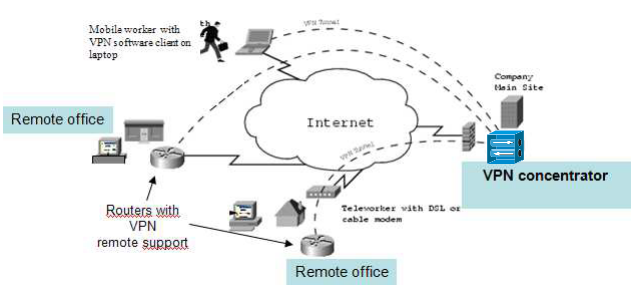
\includegraphics[scale=0.8]{figures/ex/VPN.png}
\caption{VPN IPSec}
\end{figure}
\end{center}

Risoluzione:

$S=0.01$. VPN IPSec. Accesso da remoto ad Internet e si basa sulla presenza di un \textit{VPN Concentrator} (concentratore di reti virtuali). IPSec, SSL. Meccanismi di sicurezza. Concentratore tramite VPN. Un router normale ne supporta fino ad una centinaia di VPN (Grandi aziende come CISCO, IBM). Le richieste di instaurazione arrivano secondo un processo di POISSON. $\lambda = 200\ req/h$. Inoltre $\frac{1}{\mu} = 30\ min$ (tempo medio di servizio). $m=?\ |\ \Pr\{LOSS\} < (S = 0.01)$.

M/M/m/0. Il processo degli arrivi di POISSON. Ci viene chiesto il numero di VPN contemporanee da supportare. Sistema con PERDITA (LOSS). ed ipotesi standard sui vari tempi. $m$ router. $m$ numero di VPN contemporanee. FCFS come disciplina di coda. Non c'è una coda però, quindi non conta tanto. $(\iff d=0, (e=+\infty))$.

Vogliamo utilizzare le tabelle (B di ERLANG). Il \underline{CARICO MEDIO di LAVORO} (INTENSIT\`A DI TRAFFICO) è $(\frac{\lambda}{\mu}) = (200 x 0.5) = 100 \implies (118=m)$. $S = 0.1$ (percentuale di perdita). [ERLANG] Sebbene sia in realtà una quantità adimensionata.

\newpage

\subsection{Sistemi a coda M/M/inf}

Sistema a coda costituito da un insieme illimitato di router. NON ABBIAMO FILA DI ATTESA! (Risorse illimitate). I clienti NON sono costretti a permanere in fila di attesa. Essa è quindi praticamente irrilevante. $N(t)$ al solito è il numero di clienti nel sistema a tempo $t$. Spazio degli stati di dimensione illimitata $\iff S=\{0,1,2,\ \dots\}$. Stesse ipotesi. $N(t)$  CATENA DI MARKOV a tempo continuo (CMTC), nascita e morte, con il seguente DTT:

\begin{center}
\begin{tikzpicture}[->, >=stealth', auto, semithick, node distance=2.3cm]
\tikzstyle{every state}=[fill=white,draw=black,thick,text=black,scale=0.8]
\node[state]    (0)                     {$0$};
\node[state]    (1)[right of=0]   {$1$};
\node[state]    (2)[right of=1]   {$2$};
\node[state] (d) [right of=2] {\ldots};
\node[state]    (im1)[right of=d]   {$i-1$};
\node[state]    (i)[right of=im1]   {$i$};
\node[state]    (ip1)[right of=i]   {$i+1$};
\node[state]    (ip2)[right of=ip1]  {$i+2$};
\node[state]    (d2)[right of=ip2]   {\ldots};
\path
(0) edge[bend left]     node{$\lambda$}         (1)
(1) edge[bend left]     node{$\lambda$}         (2)
    edge[bend left,below]    node{$\mu$}            (0)
(2) edge[bend left]     node{$\lambda$}           (d)
    edge[bend left,below]    node{$2\mu$}             (1)
(d) edge[bend left]         node{$\lambda$}   (im1)
	edge[bend left,below]   node{$3\mu$}          (2)
(im1) edge[bend left]       node{$\lambda$}  (i)
	  edge[bend left,below]   node{$(i-1)\mu$}     (d)
(i)   edge[bend left]   node{$\lambda$}      (ip1)
      edge[bend left,below]  node{$i\mu$}          (im1)
(ip1) edge[bend left]       node{$\lambda$}  (ip2)
	 edge[bend left,below]   node{$(i+1)\mu$}      (i)
(ip2)edge[bend left]       node{$\lambda$}  (d2)
	 edge[bend left,below]   node{$(i+2)\mu$}     (ip1)
(d2)edge[bend left,below]    node{$(i+3)\mu$}     (ip2);
\end{tikzpicture}
\end{center}

Abbiamo:

\[
	\left\{
	\begin{aligned}
	&\lambda_i=\lambda,\ i\geq 0\\
	&\mu_i=i\mu,\ i\geq 1
	\end{aligned}
	\right.
\]

Tassi di nascita $\lambda$, tassi di morte $i\mu$. Numero di stati illimitato. La CATENA è OMOGENEA, IRRIDUCIBILE. Dobbiamo vedere se è ERGODICA:

\[
	\left\{
	\begin{aligned}
	&[\pi_i = \pi_0 (\frac{\lambda}{\mu})^i \frac{1}{i!}]\\
	&[\pi_0 = \frac{1}{1+\sum_{k=1}^\infty{(\frac{\lambda}{\mu})^k \frac{1}{k!}}}]
	\end{aligned}
	\right.
\]

Anzitutto come sempre inglobiamo il termine 1 nella sommatoria dell'ultima equazione. Essa converge sempre. Abbiamo:

\[
	\pi_0 = \frac{1}{\sum_{k=0}^\infty{(\frac{\lambda}{\mu})^k \frac{1}{k!}}} = \e^{-\frac{\lambda}{\mu}}
\]

ove si è sfruttato il fatto che: $[\sum_{i=0}^\infty{x^i\frac{1}{i!}} = \e^x]$. Quindi NO CONDIZIONE DI ERGODICIT\`A. Tale serie CONVERGE SEMPRE. Converge sempre a patto che $\{\lambda,\mu\}$ siano finiti $(\iff \lambda,\mu <+\infty)$. Abbiamo:

\[
	\pi_i = \pi_0 (\frac{\lambda}{\mu})^i \frac{1}{i!} = (\frac{\lambda}{\mu})^i \frac{1}{i!}\e^{-\frac{\lambda}{\mu}},\ i\geq 0
\]

\underline{CATENA SEMPRE ERGODICA}. Non dobbiamo soddisfare nulla. Notiamo subito che riflette una DISTRIBUZIONE DI POISSON di parametro $\frac{\lambda}{\mu}$. Quindi: $[\bar{N} = (\frac{\lambda}{\mu})]$, anche se l'avrei potuto pure trovare con Little questo risultato: $\bar{N} = \lambda (\frac{1}{\mu})$. Quanto abbiamo detto vale per tempi di servizio distribuiti genericamente (\underline{\underline{M/G/$\infty$}}).
Tale sistema a coda è utilizzato per la modellazione dei tempi di propagazione. I tempi di propagazione sono considerati all'incirca costanti e pari a circa $(\sim \frac{2}{3} c)$.